
%% bare_jrnl.tex
%% V1.4b
%% 2015/08/26
%% by Michael Shell
%% see http://www.michaelshell.org/
%% for current contact information.
%%
%% This is a skeleton file demonstrating the use of IEEEtran.cls
%% (requires IEEEtran.cls version 1.8b or later) with an IEEE
%% journal paper.
%%
%% Support sites:
%% http://www.michaelshell.org/tex/ieeetran/
%% http://www.ctan.org/pkg/ieeetran
%% and
%% http://www.ieee.org/

%%*************************************************************************
%% Legal Notice:
%% This code is offered as-is without any warranty either expressed or
%% implied; without even the implied warranty of MERCHANTABILITY or
%% FITNESS FOR A PARTICULAR PURPOSE! 
%% User assumes all risk.
%% In no event shall the IEEE or any contributor to this code be liable for
%% any damages or losses, including, but not limited to, incidental,
%% consequential, or any other damages, resulting from the use or misuse
%% of any information contained here.
%%
%% All comments are the opinions of their respective authors and are not
%% necessarily endorsed by the IEEE.
%%
%% This work is distributed under the LaTeX Project Public License (LPPL)
%% ( http://www.latex-project.org/ ) version 1.3, and may be freely used,
%% distributed and modified. A copy of the LPPL, version 1.3, is included
%% in the base LaTeX documentation of all distributions of LaTeX released
%% 2003/12/01 or later.
%% Retain all contribution notices and credits.
%% ** Modified files should be clearly indicated as such, including  **
%% ** renaming them and changing author support contact information. **
%%*************************************************************************


% *** Authors should verify (and, if needed, correct) their LaTeX system  ***
% *** with the testflow diagnostic prior to trusting their LaTeX platform ***
% *** with production work. The IEEE's font choices and paper sizes can   ***
% *** trigger bugs that do not appear when using other class files.       ***                          ***
% The testflow support page is at:
% http://www.michaelshell.org/tex/testflow/



\documentclass[journal]{IEEEtran}
%


%~ \setcounter{secnumdepth}{3}
\usepackage{moreverb,url}
\usepackage{makeidx}         % allows index generation
\usepackage[percent]{overpic}
\usepackage{array} 
\usepackage{algorithm}
\usepackage[noend]{algpseudocode}
\usepackage{listings}
\usepackage{color}
\usepackage{bm}
\usepackage{booktabs}
\usepackage{multirow}
\usepackage[table]{xcolor}
\usepackage{amsfonts}
\usepackage{amsmath}

\newcommand{\fratop}[2]{\genfrac{}{}{0pt}{}{#1}{#2}}
\newcommand{\mx}[1]{\mathbf{\bm{#1}}} 				% Matrix symbol
\newcommand{\vc}[1]{\mathbf{\bm{#1}}} 					% Vector symbol
\newcommand{\degree}{\ensuremath{^\circ}}				% define the degree symbol
\newcommand{\pder}[2]{\frac{\partial#1}{\partial#2}}		% partial derivative
\newcommand{\ppder}[2]{\frac{\partial^2 #1}{\partial#2^2}}		% second partial derivative
\newcommand{\refframe}[1]{\mbox{\textless#1\textgreater}}	% to denote a reference frame
%\DeclareMathOperator*{\lexmin}{\text{lex}\!\min}			% lexmin
\DeclareMathOperator*{\argmin}{\arg\!\min}				% argmin
\DeclareMathOperator*{\argmax}{\arg\!\max}				% argmax
\DeclareMathOperator*{\st}{subject\,to}					% subject to
\DeclareMathOperator*{\minimize}{minimize}				% 
\DeclareMathOperator*{\maximize}{maximize}				% 
\DeclareMathOperator*{\find}{find}						% 
\DeclareMathOperator*{\dif}{\mathrm{d}}					% d
\DeclareMathOperator*{\half}{\frac{1}{2}}					% one half
\newcommand{\equilibriumfeasibility}[0]{\glslink{equilibrium feasible}{\textit{equilibrium feasibility}}}	% matrix
\newcommand{\contactreachability}{\glslink{contact reachable}{\textit{contact reachability}}}	% matrix
\newcommand{\mat}[1]{\ensuremath{\begin{bmatrix}#1\end{bmatrix}}}	% matrix
\newcommand{\rank}[1]{\text{rank}(#1)}							% rank
\newcommand{\diag}[1]{\text{diag}(#1)}							% diag
\newcommand{\x}{\ensuremath{\times}}
\newcommand{\spac}{\ensuremath{\quad}}						% alias for space in math environment
\newcommand{\dx}[0]{\ensuremath{\delta x}}					% dx
\newcommand{\du}[0]{\ensuremath{\delta u}}					% du
\newcommand{\DX}[0]{\ensuremath{\Delta X}}						% DX
\newcommand{\DU}[0]{\ensuremath{\Delta U}}						% DU
\newcommand{\T}[0]{\ensuremath{\top}}							% transpose symbol
\newcommand{\pinv}[0]{\ensuremath{\dagger}}					% pseudoinverse symbol
\newcommand{\Rv}[1]{\ensuremath{\mathbb{R}^{#1}}}				% set of real-valued vectors
\newcommand{\R}[2]{\ensuremath{\mathbb{R}^{#1\times #2}}}		% set of real-valued matrices
\newcommand{\Spd}[1]{\ensuremath{\mathbb{S}_+^{#1}}}			% set of symmetric positive-definite matrices
\newcommand{\card}[1]{\ensuremath{\left\vert{#1}\right\vert}}			% cardinality of a set
\DeclareMathOperator{\Tr}{Tr}							% trace
\newcommand{\Expect}{{\rm I\kern-.3em E}}				% expectation
\newcommand{\Normal}{\mathcal{N}}					% normal distribution
\newcommand{\Prob}[1]{\text{P}(#1)}						% probability

\newcommand{\Y}{\ensuremath{\mathcal{Y}}}					% 
\newcommand{\Yin}{\ensuremath{\mathcal{Y}_{in}}}					% 
\newcommand{\Yout}{\ensuremath{\mathcal{Y}_{out}}}					% 

%\algnewcommand{\algorithmicgoto}{\textbf{go to}}%
%%\algnewcommand{\Goto}[1]{\algorithmicgoto~\ref{#1}}%
%\algnewcommand{\Goto}{\algorithmicgoto\xspace}%
%\algnewcommand{\Label}{\State\unskip}

\newenvironment{definition}[1][Definition]{\begin{trivlist}
\item[\hskip \labelsep {\bfseries #1}]}{\end{trivlist}}


\newcommand{\commentt}[2]{\textcolor{#1}{\textbf{\textit{[#2]}}}} 	% make sure no comments left in the paper
%\newcommand{\commentt}[2]{}							% using this line rather than the previous one you remove all comments
\newcommand{\adnote}[1]{\commentt{blue}{AD: #1}}
\newcommand{\nmnote}[1]{\commentt{OliveGreen}{NM: #1}}

% Another method to track changes
% Examples of usage:
% - This is \added[id=per,remark={we need this}]{new} text.
% - This is \deleted[id=per,remark=obsolete]{unnecessary}text.
% - This is \replaced[id=per]{nice}{bad} text.
% To print the list of change use: \listofchanges
\usepackage{changes}	% use this for the working version
%\usepackage[final]{changes} % use this for the final version
\definechangesauthor[name={Andrea Del Prete}, color=orange]{adp}
\newcommand{\deladp}[1]{\deleted[id=adp]{#1}}
\newcommand{\addadp}[1]{\added[id=adp]{#1}}
\newcommand{\repadp}[2]{\replaced[id=adp]{#1}{#2}}
\definechangesauthor[name={Steve Tonneau}, color=blue]{st}
\newcommand{\delst}[1]{\deleted[id=st]{#1}}
\newcommand{\addst}[1]{\added[id=st]{#1}}
\newcommand{\repst}[2]{\replaced[id=st]{#1}{#2}}
\newcommand{\gls}[1]{\textit{#1}}
\newcommand{\glslink}[2]{{#2}}

%~ \usepackage[colorlinks,bookmarksopen,bookmarksnumbered,citecolor=red,urlcolor=red,draft]{hyperref}
\usepackage[colorlinks,bookmarksopen,bookmarksnumbered,citecolor=red,urlcolor=red]{hyperref}
%~ \usepackage{glossaries}

% If IEEEtran.cls has not been installed into the LaTeX system files,
% manually specify the path to it like:
% \documentclass[journal]{../sty/IEEEtran}





% Some very useful LaTeX packages include:
% (uncomment the ones you want to load)


% *** MISC UTILITY PACKAGES ***
%
%\usepackage{ifpdf}
% Heiko Oberdiek's ifpdf.sty is very useful if you need conditional
% compilation based on whether the output is pdf or dvi.
% usage:
% \ifpdf
%   % pdf code
% \else
%   % dvi code
% \fi
% The latest version of ifpdf.sty can be obtained from:
% http://www.ctan.org/pkg/ifpdf
% Also, note that IEEEtran.cls V1.7 and later provides a builtin
% \ifCLASSINFOpdf conditional that works the same way.
% When switching from latex to pdflatex and vice-versa, the compiler may
% have to be run twice to clear warning/error messages.






% *** CITATION PACKAGES ***
%
%\usepackage{cite}
% cite.sty was written by Donald Arseneau
% V1.6 and later of IEEEtran pre-defines the format of the cite.sty package
% \cite{} output to follow that of the IEEE. Loading the cite package will
% result in citation numbers being automatically sorted and properly
% "compressed/ranged". e.g., [1], [9], [2], [7], [5], [6] without using
% cite.sty will become [1], [2], [5]--[7], [9] using cite.sty. cite.sty's
% \cite will automatically add leading space, if needed. Use cite.sty's
% noadjust option (cite.sty V3.8 and later) if you want to turn this off
% such as if a citation ever needs to be enclosed in parenthesis.
% cite.sty is already installed on most LaTeX systems. Be sure and use
% version 5.0 (2009-03-20) and later if using hyperref.sty.
% The latest version can be obtained at:
% http://www.ctan.org/pkg/cite
% The documentation is contained in the cite.sty file itself.






% *** GRAPHICS RELATED PACKAGES ***
%
\ifCLASSINFOpdf
  % \usepackage[pdftex]{graphicx}
  % declare the path(s) where your graphic files are
  % \graphicspath{{../pdf/}{../jpeg/}}
  % and their extensions so you won't have to specify these with
  % every instance of \includegraphics
  % \DeclareGraphicsExtensions{.pdf,.jpeg,.png}
\else
  % or other class option (dvipsone, dvipdf, if not using dvips). graphicx
  % will default to the driver specified in the system graphics.cfg if no
  % driver is specified.
  % \usepackage[dvips]{graphicx}
  % declare the path(s) where your graphic files are
  % \graphicspath{{../eps/}}
  % and their extensions so you won't have to specify these with
  % every instance of \includegraphics
  % \DeclareGraphicsExtensions{.eps}
\fi
% graphicx was written by David Carlisle and Sebastian Rahtz. It is
% required if you want graphics, photos, etc. graphicx.sty is already
% installed on most LaTeX systems. The latest version and documentation
% can be obtained at: 
% http://www.ctan.org/pkg/graphicx
% Another good source of documentation is "Using Imported Graphics in
% LaTeX2e" by Keith Reckdahl which can be found at:
% http://www.ctan.org/pkg/epslatex
%
% latex, and pdflatex in dvi mode, support graphics in encapsulated
% postscript (.eps) format. pdflatex in pdf mode supports graphics
% in .pdf, .jpeg, .png and .mps (metapost) formats. Users should ensure
% that all non-photo figures use a vector format (.eps, .pdf, .mps) and
% not a bitmapped formats (.jpeg, .png). The IEEE frowns on bitmapped formats
% which can result in "jaggedy"/blurry rendering of lines and letters as
% well as large increases in file sizes.
%
% You can find documentation about the pdfTeX application at:
% http://www.tug.org/applications/pdftex





% *** MATH PACKAGES ***
%
%\usepackage{amsmath}
% A popular package from the American Mathematical Society that provides
% many useful and powerful commands for dealing with mathematics.
%
% Note that the amsmath package sets \interdisplaylinepenalty to 10000
% thus preventing page breaks from occurring within multiline equations. Use:
%\interdisplaylinepenalty=2500
% after loading amsmath to restore such page breaks as IEEEtran.cls normally
% does. amsmath.sty is already installed on most LaTeX systems. The latest
% version and documentation can be obtained at:
% http://www.ctan.org/pkg/amsmath





% *** SPECIALIZED LIST PACKAGES ***
%
%\usepackage{algorithmic}
% algorithmic.sty was written by Peter Williams and Rogerio Brito.
% This package provides an algorithmic environment fo describing algorithms.
% You can use the algorithmic environment in-text or within a figure
% environment to provide for a floating algorithm. Do NOT use the algorithm
% floating environment provided by algorithm.sty (by the same authors) or
% algorithm2e.sty (by Christophe Fiorio) as the IEEE does not use dedicated
% algorithm float types and packages that provide these will not provide
% correct IEEE style captions. The latest version and documentation of
% algorithmic.sty can be obtained at:
% http://www.ctan.org/pkg/algorithms
% Also of interest may be the (relatively newer and more customizable)
% algorithmicx.sty package by Szasz Janos:
% http://www.ctan.org/pkg/algorithmicx




% *** ALIGNMENT PACKAGES ***
%
%\usepackage{array}
% Frank Mittelbach's and David Carlisle's array.sty patches and improves
% the standard LaTeX2e array and tabular environments to provide better
% appearance and additional user controls. As the default LaTeX2e table
% generation code is lacking to the point of almost being broken with
% respect to the quality of the end results, all users are strongly
% advised to use an enhanced (at the very least that provided by array.sty)
% set of table tools. array.sty is already installed on most systems. The
% latest version and documentation can be obtained at:
% http://www.ctan.org/pkg/array


% IEEEtran contains the IEEEeqnarray family of commands that can be used to
% generate multiline equations as well as matrices, tables, etc., of high
% quality.




% *** SUBFIGURE PACKAGES ***
%\ifCLASSOPTIONcompsoc
%  \usepackage[caption=false,font=normalsize,labelfont=sf,textfont=sf]{subfig}
%\else
%  \usepackage[caption=false,font=footnotesize]{subfig}
%\fi
% subfig.sty, written by Steven Douglas Cochran, is the modern replacement
% for subfigure.sty, the latter of which is no longer maintained and is
% incompatible with some LaTeX packages including fixltx2e. However,
% subfig.sty requires and automatically loads Axel Sommerfeldt's caption.sty
% which will override IEEEtran.cls' handling of captions and this will result
% in non-IEEE style figure/table captions. To prevent this problem, be sure
% and invoke subfig.sty's "caption=false" package option (available since
% subfig.sty version 1.3, 2005/06/28) as this is will preserve IEEEtran.cls
% handling of captions.
% Note that the Computer Society format requires a larger sans serif font
% than the serif footnote size font used in traditional IEEE formatting
% and thus the need to invoke different subfig.sty package options depending
% on whether compsoc mode has been enabled.
%
% The latest version and documentation of subfig.sty can be obtained at:
% http://www.ctan.org/pkg/subfig




% *** FLOAT PACKAGES ***
%
%\usepackage{fixltx2e}
% fixltx2e, the successor to the earlier fix2col.sty, was written by
% Frank Mittelbach and David Carlisle. This package corrects a few problems
% in the LaTeX2e kernel, the most notable of which is that in current
% LaTeX2e releases, the ordering of single and double column floats is not
% guaranteed to be preserved. Thus, an unpatched LaTeX2e can allow a
% single column figure to be placed prior to an earlier double column
% figure.
% Be aware that LaTeX2e kernels dated 2015 and later have fixltx2e.sty's
% corrections already built into the system in which case a warning will
% be issued if an attempt is made to load fixltx2e.sty as it is no longer
% needed.
% The latest version and documentation can be found at:
% http://www.ctan.org/pkg/fixltx2e


%\usepackage{stfloats}
% stfloats.sty was written by Sigitas Tolusis. This package gives LaTeX2e
% the ability to do double column floats at the bottom of the page as well
% as the top. (e.g., "\begin{figure*}[!b]" is not normally possible in
% LaTeX2e). It also provides a command:
%\fnbelowfloat
% to enable the placement of footnotes below bottom floats (the standard
% LaTeX2e kernel puts them above bottom floats). This is an invasive package
% which rewrites many portions of the LaTeX2e float routines. It may not work
% with other packages that modify the LaTeX2e float routines. The latest
% version and documentation can be obtained at:
% http://www.ctan.org/pkg/stfloats
% Do not use the stfloats baselinefloat ability as the IEEE does not allow
% \baselineskip to stretch. Authors submitting work to the IEEE should note
% that the IEEE rarely uses double column equations and that authors should try
% to avoid such use. Do not be tempted to use the cuted.sty or midfloat.sty
% packages (also by Sigitas Tolusis) as the IEEE does not format its papers in
% such ways.
% Do not attempt to use stfloats with fixltx2e as they are incompatible.
% Instead, use Morten Hogholm'a dblfloatfix which combines the features
% of both fixltx2e and stfloats:
%
% \usepackage{dblfloatfix}
% The latest version can be found at:
% http://www.ctan.org/pkg/dblfloatfix




%\ifCLASSOPTIONcaptionsoff
%  \usepackage[nomarkers]{endfloat}
% \let\MYoriglatexcaption\caption
% \renewcommand{\caption}[2][\relax]{\MYoriglatexcaption[#2]{#2}}
%\fi
% endfloat.sty was written by James Darrell McCauley, Jeff Goldberg and 
% Axel Sommerfeldt. This package may be useful when used in conjunction with 
% IEEEtran.cls'  captionsoff option. Some IEEE journals/societies require that
% submissions have lists of figures/tables at the end of the paper and that
% figures/tables without any captions are placed on a page by themselves at
% the end of the document. If needed, the draftcls IEEEtran class option or
% \CLASSINPUTbaselinestretch interface can be used to increase the line
% spacing as well. Be sure and use the nomarkers option of endfloat to
% prevent endfloat from "marking" where the figures would have been placed
% in the text. The two hack lines of code above are a slight modification of
% that suggested by in the endfloat docs (section 8.4.1) to ensure that
% the full captions always appear in the list of figures/tables - even if
% the user used the short optional argument of \caption[]{}.
% IEEE papers do not typically make use of \caption[]'s optional argument,
% so this should not be an issue. A similar trick can be used to disable
% captions of packages such as subfig.sty that lack options to turn off
% the subcaptions:
% For subfig.sty:
% \let\MYorigsubfloat\subfloat
% \renewcommand{\subfloat}[2][\relax]{\MYorigsubfloat[]{#2}}
% However, the above trick will not work if both optional arguments of
% the \subfloat command are used. Furthermore, there needs to be a
% description of each subfigure *somewhere* and endfloat does not add
% subfigure captions to its list of figures. Thus, the best approach is to
% avoid the use of subfigure captions (many IEEE journals avoid them anyway)
% and instead reference/explain all the subfigures within the main caption.
% The latest version of endfloat.sty and its documentation can obtained at:
% http://www.ctan.org/pkg/endfloat
%
% The IEEEtran \ifCLASSOPTIONcaptionsoff conditional can also be used
% later in the document, say, to conditionally put the References on a 
% page by themselves.




% *** PDF, URL AND HYPERLINK PACKAGES ***
%
%\usepackage{url}
% url.sty was written by Donald Arseneau. It provides better support for
% handling and breaking URLs. url.sty is already installed on most LaTeX
% systems. The latest version and documentation can be obtained at:
% http://www.ctan.org/pkg/url
% Basically, \url{my_url_here}.




% *** Do not adjust lengths that control margins, column widths, etc. ***
% *** Do not use packages that alter fonts (such as pslatex).         ***
% There should be no need to do such things with IEEEtran.cls V1.6 and later.
% (Unless specifically asked to do so by the journal or conference you plan
% to submit to, of course. )


% correct bad hyphenation here
\hyphenation{op-tical net-works semi-conduc-tor}


\begin{document}
%
% paper title
% Titles are generally capitalized except for words such as a, an, and, as,
% at, but, by, for, in, nor, of, on, or, the, to and up, which are usually
% not capitalized unless they are the first or last word of the title.
% Linebreaks \\ can be used within to get better formatting as desired.
% Do not put math or special symbols in the title.
\title{An efficient acyclic contact planner for legged robot}
%
%
% author names and IEEE memberships
% note positions of commas and nonbreaking spaces ( ~ ) LaTeX will not break
% a structure at a ~ so this keeps an author's name from being broken across
% two lines.
% use \thanks{} to gain access to the first footnote area
% a separate \thanks must be used for each paragraph as LaTeX2e's \thanks
% was not built to handle multiple paragraphs
%

\author{Steve~Tonneau,~\IEEEmembership{Member,~IEEE,}
        Andrea~Del~Prete,~\IEEEmembership{Fellow,~OSA,}
        Julien~Pettr\'e,~\IEEEmembership{Fellow,~OSA,}
        Chonhyon~Park,~\IEEEmembership{Fellow,~OSA,}
        and~Nicolas~Mansard,~\IEEEmembership{Life~Fellow,~IEEE}% <-this % stops a space
\thanks{S. Tonneau, A. Del Prete and N. Mansard are with LAAS-CNRS / Universit\'e de Toulouse, France e-mail: (pro@stevetonneau.fr)}% <-this % stops a space
\thanks{J. Pettr\'e is with Inria, Rennes, France}% <-this % stops a space
\thanks{C. Park and D. Manocha are with UNC, Chapel Hill, USA}}

% note the % following the last \IEEEmembership and also \thanks - 
% these prevent an unwanted space from occurring between the last author name
% and the end of the author line. i.e., if you had this:
% 
% \author{....lastname \thanks{...} \thanks{...} }
%                     ^------------^------------^----Do not want these spaces!
%
% a space would be appended to the last name and could cause every name on that
% line to be shifted left slightly. This is one of those "LaTeX things". For
% instance, "\textbf{A} \textbf{B}" will typeset as "A B" not "AB". To get
% "AB" then you have to do: "\textbf{A}\textbf{B}"
% \thanks is no different in this regard, so shield the last } of each \thanks
% that ends a line with a % and do not let a space in before the next \thanks.
% Spaces after \IEEEmembership other than the last one are OK (and needed) as
% you are supposed to have spaces between the names. For what it is worth,
% this is a minor point as most people would not even notice if the said evil
% space somehow managed to creep in.



% The paper headers
%~ \markboth{Journal of \LaTeX\ Class Files,~Vol.~14, No.~8, August~2015}%
%~ {Shell \MakeLowercase{\textit{et al.}}: Bare Demo of IEEEtran.cls for IEEE Journals}
% The only time the second header will appear is for the odd numbered pages
% after the title page when using the twoside option.
% 
% *** Note that you probably will NOT want to include the author's ***
% *** name in the headers of peer review papers.                   ***
% You can use \ifCLASSOPTIONpeerreview for conditional compilation here if
% you desire.




% If you want to put a publisher's ID mark on the page you can do it like
% this:
%\IEEEpubid{0000--0000/00\$00.00~\copyright~2015 IEEE}
% Remember, if you use this you must call \IEEEpubidadjcol in the second
% column for its text to clear the IEEEpubid mark.



% use for special paper notices
%\IEEEspecialpapernotice{(Invited Paper)}




% make the title area
\maketitle

% As a general rule, do not put math, special symbols or citations
% in the abstract or keywords.
\begin{abstract}
% !TEX root =  ../main.tex
We present a contact planner for complex legged locomotion tasks: standing up, climbing stairs using a handrail, crossing rubble and getting out of a car. The need for such a planner was shown at the Darpa Robotics Challenge, where such behaviors
could not be demonstrated (except for egress).

Current planners suffer from their prohibitive algorithmic complexity, because they deploy a tree of robot
configurations projected in contact with the environment.
%~ computation times, due to the difficulty
%~ of generating contact postures in a high-dimensional solution space that is impossible to sample.

We tackle this issue by introducing a reduction property: the reachability condition. This condition defines
a geometric approximation of the contact manifold, which is of low dimension, presents a Cartesian topology, and can be efficiently sampled and explored.
%~ Informally, the condition verifies that the root configuration of a robot is close, but not too close to obstacles: close to allow contact creation, not too close to avoid collision. Thanks to this condition we decompose 
The hard contact planning problem can then be decomposed into two
%~ sub-problems: first, planning a guide path for the root without considering the whole-body configuration, using a sampling-based algorithm; then, generating a discrete sequence of whole-body configurations in static equilibrium along this path, using a deterministic contact-selection algorithm. 
sub-problems: first, we plan a path for the root without considering the whole-body configuration, using a sampling-based algorithm; then, we generate a discrete sequence of whole-body configurations in static equilibrium along this path, using a deterministic contact-selection algorithm. 

The reduction breaks the algorithm complexity encountered
in previous works, resulting in the first interactive
implementation of a contact planner (open source). While
no contact planner has yet been proposed with theoretical
completeness, we empirically show the interest of our framework:
in a
few seconds, with high success rates, we generate complex contact plans for various scenarios and two robots, HRP-2 and HyQ. These plans are validated either in dynamic simulations, or on the real HRP-2 robot.

%~ Our approach results from the pragmatic choice of favoring efficiency over completeness, which we justify empirically: in a
%~ few seconds, with high success rates, we generate complex contact plans for various scenarios and robots: HRP-2, HyQ, and a dexterous hand. These plans are then validated either in dynamic simulations, or on the real HRP-2 robot, thus demonstrating 
%~ the first interactive multi-contact planner.

\end{abstract}

% Note that keywords are not normally used for peerreview papers.
\begin{IEEEkeywords}
TODO
\end{IEEEkeywords}






% For peer review papers, you can put extra information on the cover
% page as needed:
% \ifCLASSOPTIONpeerreview
% \begin{center} \bfseries EDICS Category: 3-BBND \end{center}
% \fi
%
% For peerreview papers, this IEEEtran command inserts a page break and
% creates the second title. It will be ignored for other modes.
\IEEEpeerreviewmaketitle

\newcommand{\citep}[1]{\cite{#1}}	% to denote a reference frame
\newcommand{\citeauthor}[1]{\cite{#1}}	% to denote a reference frame

\section{Introduction}
% !TEX root =  ../main.tex
We consider the problem of planning an acyclic sequence of contacts describing the motion of a multiped robot in a cluttered environment. Acyclic contact planning is a particular class of motion planning where every configuration of the resulting trajectory must be in contact with the environment in order to maintain the equilibrium of the system.

Most multipedal locomotion systems focus on cyclic walking gaits \citep{Kajita03a}. However, executing
this behavior on cluttered environments is dangerous, if not impossible.
In an analysis of their participation to the Darpa Robotics Challenge, \citeauthor{atkensondarpa}
noted: ``Except for egress, no robots in the DRC Finals used
the  stair  railings  or  any  form  of  bracing.   Even  drunk  people  are  smart  enough  to  use  nearby  supports.
Full body locomotion (handholds,  bracing,  leaning against a wall or obstacles) should be easier than our
current high performance minimum contact locomotion approaches."

Indeed, the current approach to locomotion planning is to avoid obstacles as much as possible, instead of using them
to facilitate locomotion. The reason for this, as the authors state, is that ``More contacts make tasks
mechanically easier, but algorithmically more complicated for planning, and the transitions are difficult to
both plan and control[...].  We have seen very few robot planners that are  capable of  generating this  behavior."
The difficulty of addressing such a problem comes both in practice from the proximity to the obstacles (that tends to make the sampling of collision-free configuration tedious) and in theory from the foliation of the configuration space, where zero-measure manifolds intersect in a combinatorial manner \citep{simeon-manipulation-04}.

Previous contributions that embrace the combinatorial provide complete approaches, not applicable in practice because they require hours of computations \citep{conf/iser/BretlRLKA04}.
More recent successes use a local solution, resulting in more reasonable computation times (still far from real time), at the cost of dynamically inconsistent behaviors \citep{Mordatch:2012:DCB:2185520.2185539}.
Neither global nor local methods present satisfying performances, because planning simultaneously the robot trajectory and the contacts that allow
its execution is too costly. 

As suggested by \citeauthor{Bouyarmane2009}, we believe that these two tasks can be treated sequentially within a global planner, while preserving the completeness of the search.
We go further and claim that this can be done at a much smaller cost, provided that necessary and sufficient conditions for contact feasibility can be formulated for the robot trajectory.
This paper presents a geometrical representation of these conditions, and a concrete implementation of such a decoupled planner.
This implementation results from a trade-off between a necessary and a sufficient condition for feasibility, allowing us to find solutions extremely fast.
while preserving a success rate greater than TODO \% in the demonstrated scenarios.

In the remainder of this introduction, we discuss further the current state of the art. This allows us to situate more precisely our contributions.

\subsection{State of the art}

\newcommand{\Pa}{$\mathcal{P}_1$ }
\newcommand{\Pb}{$\mathcal{P}_2$ }

Additionally to robotics, acyclic motion planning is also a problem of interest in neurosciences, biomechanics, and virtual character animation.
Early contributions in the latter field rely on local adaptation of motion graphs \citep{citeulike:220163}, or ad-hoc construction of locomotion controllers \citep{Pettre:2003:LPD:846276.846313}. These approaches are intrinsically not able to adapt to new situations or discover complex behaviors in unforeseen contexts.

The issue of planning acyclic contacts was first completely described by \citeauthor{conf/iser/BretlRLKA04} in their seminal paper. The issue requires the simultaneous handling of two problems, $\mathcal{P}_1$: Planning a relevant guide trajectory for the root of the robot in $SE(3)$; and $\mathcal{P}_2$: the planning of a discrete sequence of acyclic contact configurations along the trajectory (A third nontrivial problem, $\mathcal{P}_3$, not adressed in this work, then consists in interpolating a complete motion between two postures of the contact sequence).  A key issue is to avoid combinatorial explosion when considering at the same time the possible contact configurations and the potential trajectories. This seminal paper proposes a first effective algorithm, able to handle simple situations (such as climbing scenarios), but not applicable to arbitrary environments. Following it, seve\-ral papers have applied this approach in particular situations, typically limiting the combinatorial by imposing a fixed set of possible contacts \citep{Hauser06usingmotion, stilman2010}.

Most of the papers that followed the work of \citeauthor{conf/iser/BretlRLKA04} have explored alternative formulations to handle the combinatorial issue. Two main directions have been explored. \textbf{On one hand, local optimization of both the root trajectory \Pa and the contact positions $\mathcal{P}_2$} has been used, to trade the combinatorial of the complete problem for a differential complexity, at the cost of local convergence. A complete example of the potential offered by such approaches was proposed \citep{Mordatch:2012:DCB:2185520.2185539} and successfully applied to a real robot \citep{mordatch2015}. To keep reasonable computation times, the method uses a simplified dynamic model for the avatar. Still, the computation time is far from interactive  (about 1 minute of computation for a sequence of 20 contacts). \citeauthor{DBLP:conf/humanoids/DeitsT14} propose to solve contact planning globally as a mixed integer problem, but only cyclic, bipedal locomotion is considered. Aside from the computation cost, a major drawback of these optimization based approaches is thus that they only offer local convergence when applied to acyclic contact planning.

\textbf{On the other hand, the two problems \Pa and \Pb might be decoupled} to reduce the complexity. The feasibility and interest of the decoupling is shown by \citeauthor{DBLP:conf/iser/EscandeKMG08} who manually set up a rough guide trajectory (i.e. an ad-hoc solution to $\mathcal{P}_1$). \Pb  is then addressed as the combinatorial computation of a feasible contact sequence in the neighborhood of the guide. A solution can then be found, at the cost of prohibitive computation times (several hours). Furthermore, this approach is suboptimal because the quality of the motion is conditioned by the quality of the guide trajectory,  which is not evaluated \textit{a priori}. \citeauthor{Bouyarmane2009} precisely focus on automatically computing a guide trajectory with guarantees of contact feasibility, by extending key frames of the trajectory into whole-body contact configurations in static equilibrium. Randomly sampled configurations are projected into the contact submanifold using a generalized inverse kinematics solver, a computationally expensive process (about 15 minutes are required to compute a guide trajectory in the examples presented). Moreover this explicit projection is yet an insufficient condition and does not provide strong guarantees on the feasibility of the path between two key positions in the trajectory.

It thus appears that an integrated optimization-based approach \citep{Mordatch:2012:DCB:2185520.2185539}, able to generate a locally-optimal, complete trajectory within minutes, currently outperforms
existing planners, decoupled or not. However, recent contributions are able to interpolate dynamically-feasible
trajectories between contact configurations \citep{herzog2015trajectory, Carpentier2016}. \citeauthor{Carpentier2016} are able to achieve this with real-time performances.
To generate the input contact configurations, there is a need for an efficient contact planner, able to break the combinatorial to generate discrete contact sequences rapidly. 
Such a planner holds the promise of a complete real-time multi-contact locomotion system.

\subsection{Paper contribution and organization}
This paper presents a pragmatic approach to break the complexity of multi-contact planning. With that objective in mind,
we believe that the separation between the generation of the guide trajectory and the contact sequence is the most promising direction \citep{DBLP:conf/iser/EscandeKMG08}.
However, this direction raises two theoretical questions that remain to be solved, or even to be properly formulated:
\begin{itemize}
\item The guide trajectory must guarantee the existence of a contact sequence to actuate it (This property is related to the controllability of the root actuated by the contact forces). We call this property \textit{true feasibility}. This property has not been studied yet; the only way to validate a waypoint in the trajectory is to explicitly compute the contact locations and forces, which is computationally not reasonable \citep{Bouyarmane2009}, unless the scenario is limited to cyclic, quasi-flat cases \citep{zucker2010optimization}.
\item There are infinite combinations of possible contact sequences for a given root trajectory. The selection of one particular contact sequence with interesting properties (minimum number of contact changes, robustness, efficiency or naturalness) has been studied for cyclic cases \citep{Hauser06usingmotion}, but has not been efficiently applied to cluttered environments (\citeauthor{bouyarmane:lirmm-00777727, DBLP:conf/iser/EscandeKMG08} mostly randomly picked one contact sequence, leading to possibly very tedious transitions.
\end{itemize}

By tackling these issues, our method proposes contributions to both problems \Pa and \Pb.
For each problem, we introduce an original formulation of the related theoretical issues.
Then, we propose a concrete implementation of the solution, where the constraints of the problem are relaxed in favor of efficiency.
The relaxation is justified empirically, with statistics presented for 2 robots and 4 scenarios. The complete framework is implemented within
the open-source platform HPP.

\begin{figure*}
  \centering
  \begin{overpic}[width=0.8\linewidth]{figures/workflow}
    %~ \put (6.4,1.8) {\normalsize{Request}} 
    \put (30,10.8) {\large{\color{white}\Pa} }
    %~ \put (31.6,2) {\scriptsize{\color{white}RB-RRT}} 
    \put (66.4,10.8) {\large{\color{white}\Pb} }
    %~ \put (72.5,2) {\tiny{\color{white}Contact}} 
  \end{overpic}
  \vspace{-1em}
  \caption{
    Overview of our 2-stage framework. \Pa: Given a path request between the yellow and blue positions, a guide path is computed in the space of truly feasible guides $C_{reach}$. This is achieved by defining a geometric condition, the reachability condition (abstracted here with the transparent cylinders). \Pb: The trajectory is extended into a discrete sequence of contact configurations using an iterative algorithm.}
  \label{fig:framework}
\end{figure*}

To address \Pa we rigorously formulate a geometric condition that approximates the true feasibility of a path, the reachability condition. We claim that this 
condition can be verified in a low-dimensional space, which we call $C_{reach}$. This formulation can make the planning of a guide path more efficient computationally, while providing similar guarantees to planning directly in the configuration space.
In practice, for each considered robot, we compute an approximation of $C_{reach}$. From this approximation,
an efficient trade-off between a necessary and a sufficient condition for true feasibility is obtained. This trade-off allows the implementation of a low-dimensional, Reachability-Based RRT planner (RB-RRT), able to find truly-feasible paths for the root of the robot in a timespan ranging from a few milliseconds to a few seconds, depending on the scenario.

To address \Pb, we consider a truly-feasible path as an input, and generate new contact configurations along it using a sampling approach.
The true feasibility of the path provides guarantees that the contacts can be created, and reduce the dimensionality of the problem (at each step the root position is fixed). The theoretical completeness of the approach is partially traded for efficiency: instead of sampling online
limb configurations and projecting them onto contact, we precompute offline a large database of limb configurations, stored in a spatial structure optimized
for proximity queries. At runtime, this framework allows to obtain rapidly a set of candidate configurations for contact.
These candidates are sorted using a criterion to evaluate the static equilibrium of the configuration, as well as a set of user-defined heuristics.
In all our experiments we used two such heuristics: a measurement of robustness of a configuration to errors in the contact forces, and a manipulability-based heuristic,
the Extended FORce Transmission ratio (EFORT).

The contribution of the paper is thus twofold. We propose a theoretical characterization of today's most efficient practical approach to sampled-based planning of acyclic contacts. Based on this characterization, we propose a very efficient and general implementation of an acyclic contact planner, the first one compatible with interactive applications.

Compared to previous work \citep{Mordatch:2012:DCB:2185520.2185539} our planner does not produce a complete motion, but a discrete sequence of contacts.
Since the interpolation of a complete trajectory between such configurations can be solved within real-time constraints \citep{Carpentier2016}, we claim that our planner
is the fastest multi-contact planning solution to our knowledge.

The present paper is an extension of a conference paper to appear in the proceedings of the ISRR'15 conference~\citep(tonneauisrr15).
The conference paper focuses on the theoretical formulation of the problem, and presents results obtained with virtual avatars.
This extension completes this work with a discussion on the implementation of this theory to real-world robots and problems.
In particular, we introduce a robust balance criterion, designed to ensure the equilibrium of the robot despite bounded error in the contact forces. We also provide details on the HPP implementation
of our contact generation algorithm. Furthermore, our experiments are now applied to real-robot models, namely HRP-2 and HyQ\adnote{cite Semini}. Appendix~\ref{app:rom} describes the generation process
for the robot.

In Section~\ref{overview}, we present the general organization of our method. Section~\ref{rbprm} and Section~\ref{sec:contact} present respectively our answer to \Pa and \Pb. In Section~\ref{sec:heuristics}, we present two heuristics used for the selection of a contact configuration. Finally, we propose a complete experimental validation of the planner with three very different kinematic chains (the HRP-2 and HyQ robots, and a three-finger manipulator) in various scenarios,
that complete those presented in the conference paper.

% !TEX root =  ../main.tex
\section{Overview}
\label{overview}

Figure~\ref{fig:framework} illustrates our workflow.
\Pa and \Pb are addressed in a sequential fashion.
The guarantees provided by the truly-feasible guide path allow
us to avoid the combinatorial by generating the contacts in a straightforward manner.



%
\begin{figure*}
  \centering
  \begin{overpic}[width=0.8\linewidth]{figures/contact_gen}
		\put (1,1) {1} 
		\put (22,1) {2} 
		\put (42,1) {3} 
		\put (62,1) {4} 
		\put (83,1) {5} 
	\end{overpic}
  \caption{Generation of a contact configuration for the right leg of HRP-2. 1: Selection of reachable obstacles. 2: Entries of the limb samples database (with $N = 4$). 3: With a proximity query on the octree database, configurations too far from obstacles are eliminated. 4: The best candidate according to a user-defined heuristic $h$ is chosen. 5: The final contact is achieved using inverse kinematics.}
  \label{fig:contact_gen}
\end{figure*}
\subsection{Computation of a guide path --- \Pa}
We first consider the problem of planning a relevant guide path. The objective is to compute a path of root placements which will allow contact creation. A desired requirement is to preserve the completeness of the planner: it should be able to explore any possible guide trajectory, but at the same time, any computed guide trajectory must be truly feasible, i.e. must lead to a valid sequence of contacts.

 An intuitive description of such placements is ``close, but not too close'': close, because a contact surface must be partially included in the Reachable workspace of the robot (represented for the right arm in Fig.~\ref{fig:contact_gen}--1); not too close, because the robot must avoid collision (which is represented by the hull including the torso in Fig.~\ref{fig:contact_gen}--1). We define formally $C_{reach}$, the set of interesting \adnote{'interesting' is vague, consider replacing with 'the set of root placements that allow the robot not to be in collision and be in contact with the environment'; alternatively you can even be more precise I write this in math, but maybe that's not the right place to be formal}  root placements, in which we compute a guide trajectory with a sampling based planner,  the Reachability-Based RRT --RB-RRT-- (Figure~\ref{fig:framework}--\Pa). Planning in $C_{reach}$ boils down to planning in SE(3), which has an acceptable practical complexity.
%
Details are presented in Section~\ref{rbprm}.

\subsection{Generating a discrete sequence of contact configurations --- \Pb}

The second stage extends the guide path into a sequence of contact configurations (Fig.~\ref{fig:framework}--\Pb). The true feasibility of the input path is guaranteed by the first step.
This provides in turn a reasonable \adnote{FYI: you always wrote 'reasonable' as 'reasonnable'} guarantee that a contact configuration can be obtained for any root placement along the path. With a fixed root position, the dimensionality of the 
contact generation problem is reduced to the number of degrees of freedom of the considered limb. In other words, we consider each limb as a manipulator attached to the root, and select the most relevant contact from a database of precomputed configurations, which is independent from the environment (Figure~\ref{fig:contact_gen}).

From a given start configuration, the planner proceeds in an iterative fashion along the discretized path: given a new root placement, an inverse-kinematics solver 
is used to maintain the contacts that were previously existing (TODO Figure). Often, these contacts cannot be maintained, because of joint limits or collisions (TODO Figure).
In such a case the contacts are broken. Conversely, new contacts are created to ensure the static equilibrium of the robot (TODO FIGURE).
The algorithm is designed so that only one contact can be created or broken between two successive configurations. This can be seen as a heuristic \adnote{why heuristic?} to ensure
that the interpolation between two configurations is achievable.
Details are presented in Section~\ref{sec:efort}. 

To select the ``most relevant'' contact configurations, user-defined heuristics can be chosen. In Section~\ref{heuristics} we present extensively two such heuristics, that have been
used in our experiments.


%~ To create a contact, we consider each limb of the robot as a manipulator arm attached to the root. We store a database of configurations for each manipulator. Figure~\ref{fig:contact_gen} -- 2 presents a few configurations for the right arm of the robot. The configurations in the database which are close to contact are considered (Figure~\ref{fig:contact_gen} -- 2 and 3). Among the candidates, 3 criteria are considered to choose the most relevant: the ideal candidate is free of collision, allows to maintain static balance if necessary, and  contributes to the motion in an optimal way. We call the measure of this contribution task efficiency: it represents the ability the limb has to exert a force compatible with the direction of motion. In Figure~\ref{fig:contact_gen} -- 4, the black arrow represents the direction of motion. Among the candidates, the most relevant to achieve a vertical motion is chosen, and projected on the contact surface using an inverse kinematics solver (Figure~\ref{fig:contact_gen} -- 5). The task efficiency is measured using the Extended FORce Transmission ratio (EFORT), proposed by ~\cite{Tonneau:2014:TEC:2619648.2619652}.

\subsection{Notation conventions and definitions} \label{notations}

A vector  $\mathbf{x}$ is denoted with a bold lower-case letter.
A matrix $\mathbf{A}$ is denoted with a bold upper-case letter.
A set $C$ is denoted with an upper-case italic letter.
Scalar variables and functions are denoted with lower-case italic letters, such as
$r$ or $f(\textbf{x})$.

%\subsubsection{Robot description}
%\label{def}

\begin{figure}
  \centering
  \begin{overpic}[width=0.8\linewidth]{figures/character}
    \put (7,29) {\small{$\in \mathbf{q}^1$}}
    \put (7,25) {\small{effector}}
  \end{overpic}
  \caption{
    Left: Robot in a rest configuration. The right arm is denoted as the limb $R^1$. Each colored dot represents a degree of freedom around an axis. Right: Volumes of the robot. The red geometry denotes $W^0$ and must remain collision-free. The green spheres are the reachable workspace of each limb, the  $W^k$.}
  \label{fig:character}
\end{figure}

\medskip
\textbf{A robot} is a kinematic chain $R$, comprising \mbox{$n + 6$} degrees of freedom (DOFs).
$R$ is composed of $l$ limbs $R^k, 1 \leq k \leq l$, attached to a root.
It is described by a configuration $\mathbf{q} \in SE(3) \times \mathbb{R}^n$.
We define some relevant projections of $\mathbf{q}$:
\begin{itemize}
	\item $\mathbf{q}^k$ denotes the configuration (a vector of joint values) of the limb $R^k$ (Fig.~\ref{fig:character});
	\item $\mathbf{q}^{\overline{k}}$ denotes the vector of joint values of R \textbf{not} related to $R^k$. We define for convenience \mbox{$\mathbf{q}= \mathbf{q}^k \oplus \mathbf{q}^{\overline{k}}$}; %Abusively, we denote by $\mathbf{q}^0 \oplus \mathbf{q}^k$ any configuration respecting $\mathbf{q}^0$ and $\mathbf{q}^k$;
	\item $\mathbf{q}^{0}\in SE(3)$ denotes the position and orientation of the root of the robot $R$.
\end{itemize}
%Finally, $ \mathbf{q}_{start}$ and  $\mathbf{q}_{goal}$ are the start and goal configurations given as an input of our problem.

%\subsubsection{Environment and other volumes} 
%\label{sec:A}
\medskip
The volume encompassing the trunk of the robot is denoted $W^0$ (Fig.~\ref{fig:character}-right: central cylinder). The reachable workspace of a limb $R^k$ is denoted $W^k$ (Fig.~\ref{fig:character}-right: the four ellipses). 
\begin{equation}
  W^k = \left\{ {\mathbf{x} \in \mathbb{R}^3: \exists \, \mathbf{q}^k, \mathbf{p}^k(\mathbf{q}^k) = \mathbf{x} } \right\},
\end{equation}
\adnote{in this definition you don't account for joint limits}
where $\mathbf{p}^k$ denotes the end-effector position of $R^k$ (translation only) for $\mathbf{q}^0$ being the null displacement. We also define $W = \bigcup_{k=1}^{l}W^k$, and
$W^k(\mathbf{q}^{0})$ (for $1 \leq k \leq l$) as the volume $W^k$ translated and rotated by the rigid displacement~$\mathbf{q}^{0}$.

\medskip
\textbf{The environment} $O$ is defined as the union of the obstacles $O_i$ that it contains.
Finally, we define $dist(\mathbf{x}, O)$ as the minimal distance between a point $\mathbf{x}$ and the closest surface of the environment.

% !TEX root =  ../main.tex
%~ \section{Computing a guide path in $C^0_{reach}$ ($\mathcal{P}_1$) }
\section{Root path planning in the contact reachable space}
\label{rbprm}

During the root path planning we only consider the root configuration $\mathbf{q}^0$ defined in the previous Section,
as well as the environment $O$.

Given a start and a goal configurations, we aim at computing a guide path $\mathbf{q}^0(t) : [0,1] \longrightarrow$ $\mathbb{R}^r$ verifying:
\begin{equation*} \label{eq:path}
\forall t \in [0,1], \mathbf{q}^0(t)  \in C_{Equil}^0
\end{equation*}
This means that any root configuration must be extended into a whole-body, static equilibrium configuration.
$C_{Equil}^0$  cannot be described analytically.

The strong hypothesis of this work is that for a large variety of locomotion tasks, we can define a space  $C_{Reach}^0 \simeq C_{Contact}^0$, such that 
\begin{equation} \label{eq:creach}
\forall t \in [0,1], \mathbf{q}^0(t) \in C_{Reach}^0 \Rightarrow \mathbf{q}^0(t)  \in C_{Equil}^0
\end{equation}
% for \gls{cluttered} problems.
We call  $C_{Reach}^0$ the \textit{contact reachable workspace}, and detail its construction in the following.
The validity of this hypothesis is discussed in depth in Section~\ref{sec:discussion}.
%~ We describe the construction of $C_{Reach}^0$ in the following.
 
\subsection{Conditions for contact reachability}
The contact reachable workspace is defined as a compromise between two necessary and a sufficient condition for contact creation.

\textbf{necessary conditions:}
For a contact to be possible, an obstacle $O_i \subset O$ necessarily intersects the reachable workspace $W(\mathbf{q}^{0})$ of the robot (Figure~\ref{fig:contact_gen}--1). Also the torso of the robot $W^0(\mathbf{q}^{0})$ must necessarily be collision-free.
Therefore we can define an outer approximation  $ \mathcal{C}^0_{\textrm{\it Nec}} \supset$ $C_{Contact}^0$ as: 
\begin{equation}
\mathcal{C}^0_{\textrm{\it Nec}} = \{ \mathbf{q}^0 : W(\mathbf{q}^{0}) \cap O \neq \emptyset \textrm{ \textbf{and}}\ W^0(\mathbf{q}^{0}) \cap O = \emptyset \} % \\ }
 %~ & \text{ and } & A_{torso}(\mathbf{q}^{root}) \cap W = \emptyset \}
\end{equation}
%~ The inclusion $C_{Contact}^0$ $\subset \mathcal{C}^0_{\textrm{\it Nec}}$ is straightforward, but it is very important.
%~ Planning in $\mathcal{C}^0_{\textrm{\it Nec}}$ allows a strong reduction of the search space, while not discarding 
%~ any root configuration that could lead to a solution.
 
%~ The condition defining $\mathcal{C}^0_{\textrm{\it Nec}}$ is only necessary. This means that it might not be possible to extend a guide path planned 
%~ in $\mathcal{C}^0_{\textrm{\it Nec}}$ into a sequence of contact configurations.

\textbf{sufficient condition:}
Similarly we can define an inner approximation \mbox{$\mathcal{C}^0_{\textrm{\it Suf}} \subset $ $C_{Contact}^0$} by considering a bounding volume $B^{\textrm{\it Suf}}$ encompassing the whole robot in a given pose, except for the effector surfaces. 
\begin{equation}
\mathcal{C}^0_{\textrm{\it Suf}} = \{ \mathbf{q}^0 : W(\mathbf{q}^{0}) \cap O \neq \emptyset \textrm{ \textbf{and}}\ B^{\textrm{\it Suf}}(\mathbf{q}^{0}) \cap O = \emptyset \} % \\ }
 %~ & \text{ and } & A_{torso}(\mathbf{q}^{root}) \cap W = \emptyset \}
\end{equation}

%~ In general, the inclusion is strict, which means that we lose the completeness of the two-stage contact planner (i.e. the planner is not able to discover a path inside \mbox{$C_{reach} \setminus \mathcal{C}^0_{\textrm{\it Suf}}$}). However, the sufficient condition guarantees that any such path leads to a valid sequence of contacts.

\subsection{The compromising reachability condition}
\label{sec:scaling}
The ideal shape $B^*, W^0 \subset B* \subset B^{\textrm{\it Suf}}$ that defines a necessary \textbf{and} sufficient condition for contact creation has no explicit definition.
Therefore, we approximate $B^*$ to define the contact reachable space $C_{Reach}^0$.

%~ However, using a shape between $W^0$ and $B^{\textrm{\it Suf}}$ leads to a trade-off between a necessary and a sufficient condition. 
We define $W^0_s$ as the volume $W^0$ subject to a scaling transformation by a factor $s \in \mathbb{R}^+$.
%
We then consider the spaces $C_{s}^0$
 \begin{equation}
 \label{eq:reachc}
C^0_s = \{ \mathbf{q}^0 : W(\mathbf{q}^{0}) \cap O \neq \emptyset \textrm{ \textbf{and}}\ W^0_s(\mathbf{q}^{0}) \cap O = \emptyset \} % \\ }
 %~ & \text{ and } & A_{torso}(\mathbf{q}^{root}) \cap W = \emptyset \}
\end{equation}
%
The parametrization of $s$ defines a trade-off:
If $s=1$, then $W^0_s$ = $W^0$, such that $C_1^0$ = $\mathcal{C}^0_{\textrm{\it Nec}}$.
 %~ We thus consider that $s \geq 1$, since smaller values would only worsen the approximation.
By increasing $s$, the condition can become sufficient, but less and less necessary.  
Eq.~\ref{eq:reachc} thus defines the \textit{reachability condition}. We fix a value $s^*$ for $s$ and define  $C_{Reach}^0 = C^0_{s^*}$.
The computation of $s^*$ is detailed in Section~\ref{sec:params}. 
In Appendix~\ref{app:rom}, we give a generic method to compute the $W$ volumes appearing in the definition of $C_{Reach}^0$.

\subsection{Computing the guide path in $C_{reach}^0$}
$C_{Reach}^0$ can be sampled efficiently thanks to Eq.~\ref{eq:reachc}, and can thus be used with any standard motion planner.
%~ The only significant change is to replace the collision checking with the \textit{reachability condition}.
Our current implementation uses the Bi-RRT planner \citep{770022} provided by the HPP software~\citep{7759083}.
Our implementation is exactly the same as the pseudo-code of the original planner (which does not detail the configuration validation method). With respect to a ``classic'' implementation, the only difference is that instead of validating a configuration using collision detection, we validate it with the \textit{reachability condition}.\\

%~ \delst{However, to improve the sampling efficiency 
%~ we bias the sampling process to generate near-obstacle configurations, similarly to cite{Amato98choosinggood}.}

This Section has presented a guide path planner for the geometric root of a robot, implemented as a low-dimensional sampling-based 
algorithm. Given start and goal configurations, it outputs a continuous path for the robot's root. 
%~ \deladp{Thanks to the \textit{reachability condition}, we assume that for any configuration in the path there exists a joint configuration that results in static equilibrium.}
%~ Thanks to these modifications, the problem of planning a \gls{contact reachable} path is reduced to a geometric collision-checking problem, of low dimension (6 for HyQ, 8 for HRP-2 that has 2 joints in the torso).
%~ By doing this we can solve the problem with a sampling-based approach, in \gls{interactive} computation times.

% !TEX root =  ../main.tex
\section{From a guide path to a discrete sequence of contact configurations ($\mathcal{P}_2$)}
\label{sec:contact}
As an input of this stage, we consider a \textit{geometrically feasible} guide path $\mathbf{q}^0(t) : [0,1] \longrightarrow SE(3)$ for the root of the robot $R$. We now consider the second problem of computing a discrete sequence of contact configurations $\mathbf{Q}^{\overline{0}}$ for the limbs of the robot along $\mathbf{q}^0(t)$.

In this Section we first describe a single contact-generation process, that is how to generate a contact configuration for a given limb 
and root location.
Then, on this method we build an iterative algorithm to generate a discrete sequence of contact configurations in equilibrium.

In what follows a \textit{valid} contact configuration is understood as being collision free, satisfying joint limits, and allowing to maintain the static equilibrium
of the robot. The first two tests are trivial; our criterion to assert efficiently the static equilibrium of the system
is described in Section~\ref{sec:heuristics}.

\subsection{Definition of a contact generator}
\label{sec:single_contact}
We consider a limb $R^k$  and a root configuration $\mathbf{q}^0$.
From \textit{geometrical feasibility} we know that there exists an infinite list of mappings $P = [\pi_0,..,\pi_i, ...]$ that verify \eqref{eq:pi} for $\mathbf{q}^0$.
The issue is then to evaluate locally at least one element of $P$ at $\mathbf{q}^0$.

While exhibiting analytically a $\pi_i$ does not seem tractable, we can iteratively evaluate $\pi_i(\mathbf{q}^0)$ as follows:
\begin{enumerate}
\item Generate randomly a collision-free limb configuration;
\item Project the end-effector onto the closest surface with inverse kinematics;
\item If a valid solution is found, stop. Otherwise repeat from step 1.
\end{enumerate}


We partially trade the completeness property of this approach for a more efficient solution introduced in our previous work~\citep{Tonneau2014}, which we describe
here for completeness.

We first define $C_{Contact}^{\epsilon} \supset C_{Contact}$ as the set of configurations almost in contact. This means that the minimal distance 
between an effector and a surface of the environment is less than a small value $\epsilon$.
We then apply the following steps:
\begin{enumerate}
\item Generate off-line $N$ valid sample limb configurations $\mathbf{q}^k_i,  0 \leq i < N$;
\item Using the end-effector positions $\mathbf{p}(\mathbf{q}^k_i)$ as indices, store each sample in an octree data structure;
\item Figure~\ref{fig:contact_gen}--b and c--: At runtime, when contact creation is required, retrieve from the octree the list of samples $S \subset C_{Contact}^{\epsilon}$ close to contact;
\item According to a user-defined heuristic $h$, sort the elements of $S$;
\item Figure~\ref{fig:contact_gen}--d and e--: Select the first configuration of $S$ (or fail if $S$ is empty). Project the configuration onto contact with inverse kinematics;
\item If a valid solution is found, stop. Otherwise remove the element from $S$ and go back step 5.
\end{enumerate}

This approach has two main advantages.
First, this allows us to select a large number of candidates in a single proximity request.
Having several candidates is interesting, because it allows to compare them using a user-selected heuristic $h$, thus obtaining
a locally-optimal candidate.
Furthermore, the fact that the candidates are already close to contact increases the odds that the inverse kinematics will converge to a valid solution in a small number of iterations.
Regarding completeness, it is immediate to verify that as $N$ grows, the completeness of the method is restored.
$N$ is a parameter that allows us to specify the trade-off between completeness and efficiency.
The reader is invited to refer to our previous work for an extensive discussion on the optimal value of $N$ \citep{Tonneau2014}.

We thus have defined a real-time contact generator. For a given configuration, the generator can be as complete as required by the context (by increasing the number of samples).

\subsection{Extension of the guide trajectory}
Using the contact generator, we define an iterative algorithm to generate the contact
sequence along the guide path.
Although we address acyclic contact sequences, the algorithm is deterministic in the order in which 
the contacts are created, allowing it to break the combinatorial.
The complete algorithm can be found in Appendix~\ref{app:contact}.
In the remainder of the section we provide an intuition of it.

As an input, we consider the guide path $\mathbf{q}^0(t)$, automatically discretized into a sequence of $j$ key placements:  
\begin{equation*}
	\mathbf{Q}^0 = [\mathbf{q}^0_{0}; \mathbf{q}^0_{i}; ..., \mathbf{q}^0_{j-1}]
\end{equation*} 
where $\mathbf{q}^0_{0}$ and $\mathbf{q}^0_{j-1}$ respectively correspond to the start and goal configurations. To ensure continuity in the contact transition phases, we rewrite $\pi$ under the following recursive form for any $0<i<j$:
\begin{equation*}
    \pi\colon\left\{
    \begin{aligned}		
        \mathbf{Q}^0 \in C_{reach} & \longrightarrow C_{contact} \\
        %\mathbf{q}^{0}_0 &  \longrightarrow  \mathbf{q}_{start} \\
        \mathbf{q}^{0}_i &  \longrightarrow  \mathbf{q}^{0}_i \oplus g(\mathbf{q}_{i - 1},\mathbf{q}^{0}_i) 
    \end{aligned}
    \right.
\end{equation*} 
$g$ is the method that extends a root configuration into a full-body configuration. At each step, it tries to generate a contact configuration that preserves as much as possible
the previous contacts while allowing for static equilibrium. The objective is thus to characterize $g$.
We initialize the recurrence with $\pi(\mathbf{q}^0_{0}) = \mathbf{q}_0$ the initial configuration of the robot.

%~ The function $g$ is defined independently by $g^k$ for each limb $R^k$. In defining $g^k$, two aspects must be considered. Is the limb $R^k$ in contact? And which criteria is it optimizing? 

\subsubsection{Maintaining a contact in the sequence.}

Figure~\ref{fig:break_contact} illustrates the contact-persistence strategy.
If possible, a limb in contact at time $i-1$ remains in contact at time $i$. The contact is broken if an inverse-kinematics solver fails to find a collision-free limb configuration that satisfies joint limits. The solver is directly provided by the HPP software.

If the solver fails, the contact is broken and a collision-free configuration is assigned to the limb.
If two or more contacts are broken in a single time step, intermediate steps are added to reposition the contacts one at a time, before moving.

\begin{figure}[t]
\centering
  \begin{overpic}[width=0.9\linewidth]{figures/break_contact}
		\put (0,4) {1} 
		\put (25,4) {2} 
		\put (50,4) {3} 
		\put (76,4) {4} 
		%~ \put (68,58) {3.a)} 
		%~ \put (5,27) {3.b)} 
		%~ \put (37,27) {4.a)} 
		%~ \put (68,27) {4.b)} 
	\end{overpic}
\caption{Contacts are maintained if joint limits and collisions constraints are respected (2). They are broken otherwise(3,4).}
		   \label{fig:break_contact}
\end{figure}

%~ \begin{figure}[t]
%~ \centering
  %~ \begin{overpic}[width=0.6\linewidth]{figures/generate_contact}
		%~ \put (5,58) {1)} 
		%~ \put (37,58) {2)} 
		%~ \put (68,58) {3.a)} 
		%~ \put (5,27) {3.b)} 
		%~ \put (37,27) {4.a)} 
		%~ \put (68,27) {4.b)} 
	%~ \end{overpic}
%~ \caption{Contacts are generated when the configuration is not balanced.}
		   %~ \label{fig:generate_contact}
%~ \end{figure}

%\subsection{Generation of a contact configuration}  
\subsection{Creating contacts.}
Contacts are created using three rules:
\begin{enumerate}
\item Only one contact creation can happen between two consecutive states. This increases the odds that the interpolation between the two states be feasible;
%\adnote{Before you said that you ensured that transition between two states is feasible...}
\item A contact is validated if and only if the resulting configuration is in static equilibrium, no matter what user-defined heuristics are used; 
\item We use a FIFO approach:  we always try first to create a contact with the limb that has been contact-free the longest. If the contact creation
was not successful for a limb, the limb is pushed on top of the queue, and will only be tried again after the others have been treated.
\end{enumerate}

These three rules provide a deterministic manner to generate contacts along the discretized guide path.
For a given truly feasible path, our current implementation does not guarantee that the planner will succeed in generating a configuration in static equilibrium, because
of the deterministic approach used to break the combinatorial.
However, in practice the planner is successful in the large majority of cases, as discussed in Section~\ref{sec:perf}, thanks to 
the heuristics that we use for contact selection.

% !TEX root =  ../main.tex
\section{Results}
\label{sec:results}
In this section we present some of the results obtained with our planner. The complete sequences are shown in the companion video.
Specifically, we demonstrate the planner for two legged robots, in a large variety of environments: the humanoid HRP-2 and the quadruped HyQ.
Finally, a last example suggests possible applications to dexterous manipulation.

At the end of the video, we validate our contact plans by exhibiting a solution to the interpolation problem $\mathcal{P}_3$ for these scenarios.

At the end of this section, we discuss the role of the parameters of our framework. We then provide the \textit{interactive} computation times obtained in each case.
We also compare the times obtained with HRP-2 with respect to previous works.

These scenarios complement the ones demonstrated on virtual avatars (Figure~\ref{fig:robots_old}) in our previous ISRR paper~\citep{tonneauisrr15} and video\footnote{\url{http://youtu.be/LmLAHgGQJGA}}.
%~ (Figure~\ref{fig:robots_old}).
 %~ We invite the interested reader to watch the ISRR video (\url{http://youtu.be/LmLAHgGQJGA}), and 
%~ to refer to the previous paper for a discussion on these results.

%~ We say that the planning is \gls{interactive} when the computation time for one step is lesser than the
%~ time to execute it. We arbitrarily approximate this time to one second.

\begin{figure}[t]
\centering
  \begin{overpic}[width=1\linewidth]{figures/robots_old}
		%~ \put (5,) {1)} 
		%~ \put (37,) {2)} 
		%~ \put (68,) {3.a)} 
		%~ \put (5,27) {3.b)} 
		%~ \put (37,27) {4.a)} 
		%~ \put (68,27) {4.b)} 
	\end{overpic}
\caption{Virtual avatars in various scenarios demonstrated in our conference paper.}
		   \label{fig:robots_old}
\end{figure}

\subsection{Description of the scenarios}
In all the scenarios considered, the formulation of the problem is always the same:
a start and goal root configurations are provided as input.
The framework computes the initial contact configuration, and outputs a sequence of contact configurations connecting it to the goal.
In each scenario we detail the contacts involved and the heuristics chosen (either $h_{\textrm{\it EFORT}}$, $h_{vel}$ or $h_{w}$, all of which are defined in the Appendix~\ref{sec:heuristics}).
 %~ and the constraints on the reachable workspaces (for instance in all the scenarios, the reachable workspaces of the legs of HRP-2 are always required to intersect with the environment). 
%~ The companion video presents the complete contact sequence obtained in all these scenarios.

% \subsubsection*{Truck egress (Figure~\ref{res_truck_pres} and Figure~\ref{res_truck_bd}) -- Humanoid and insectoid robots.}
%\subsubsection*{Truck egress -- Humanoid and insectoid robots (Figure~\ref{res_truck_bd}).}
\subsubsection{HRP-2 -- Steep staircase (Figure~\ref{fig:stair_robust}):}

\begin{figure}
  \centering
  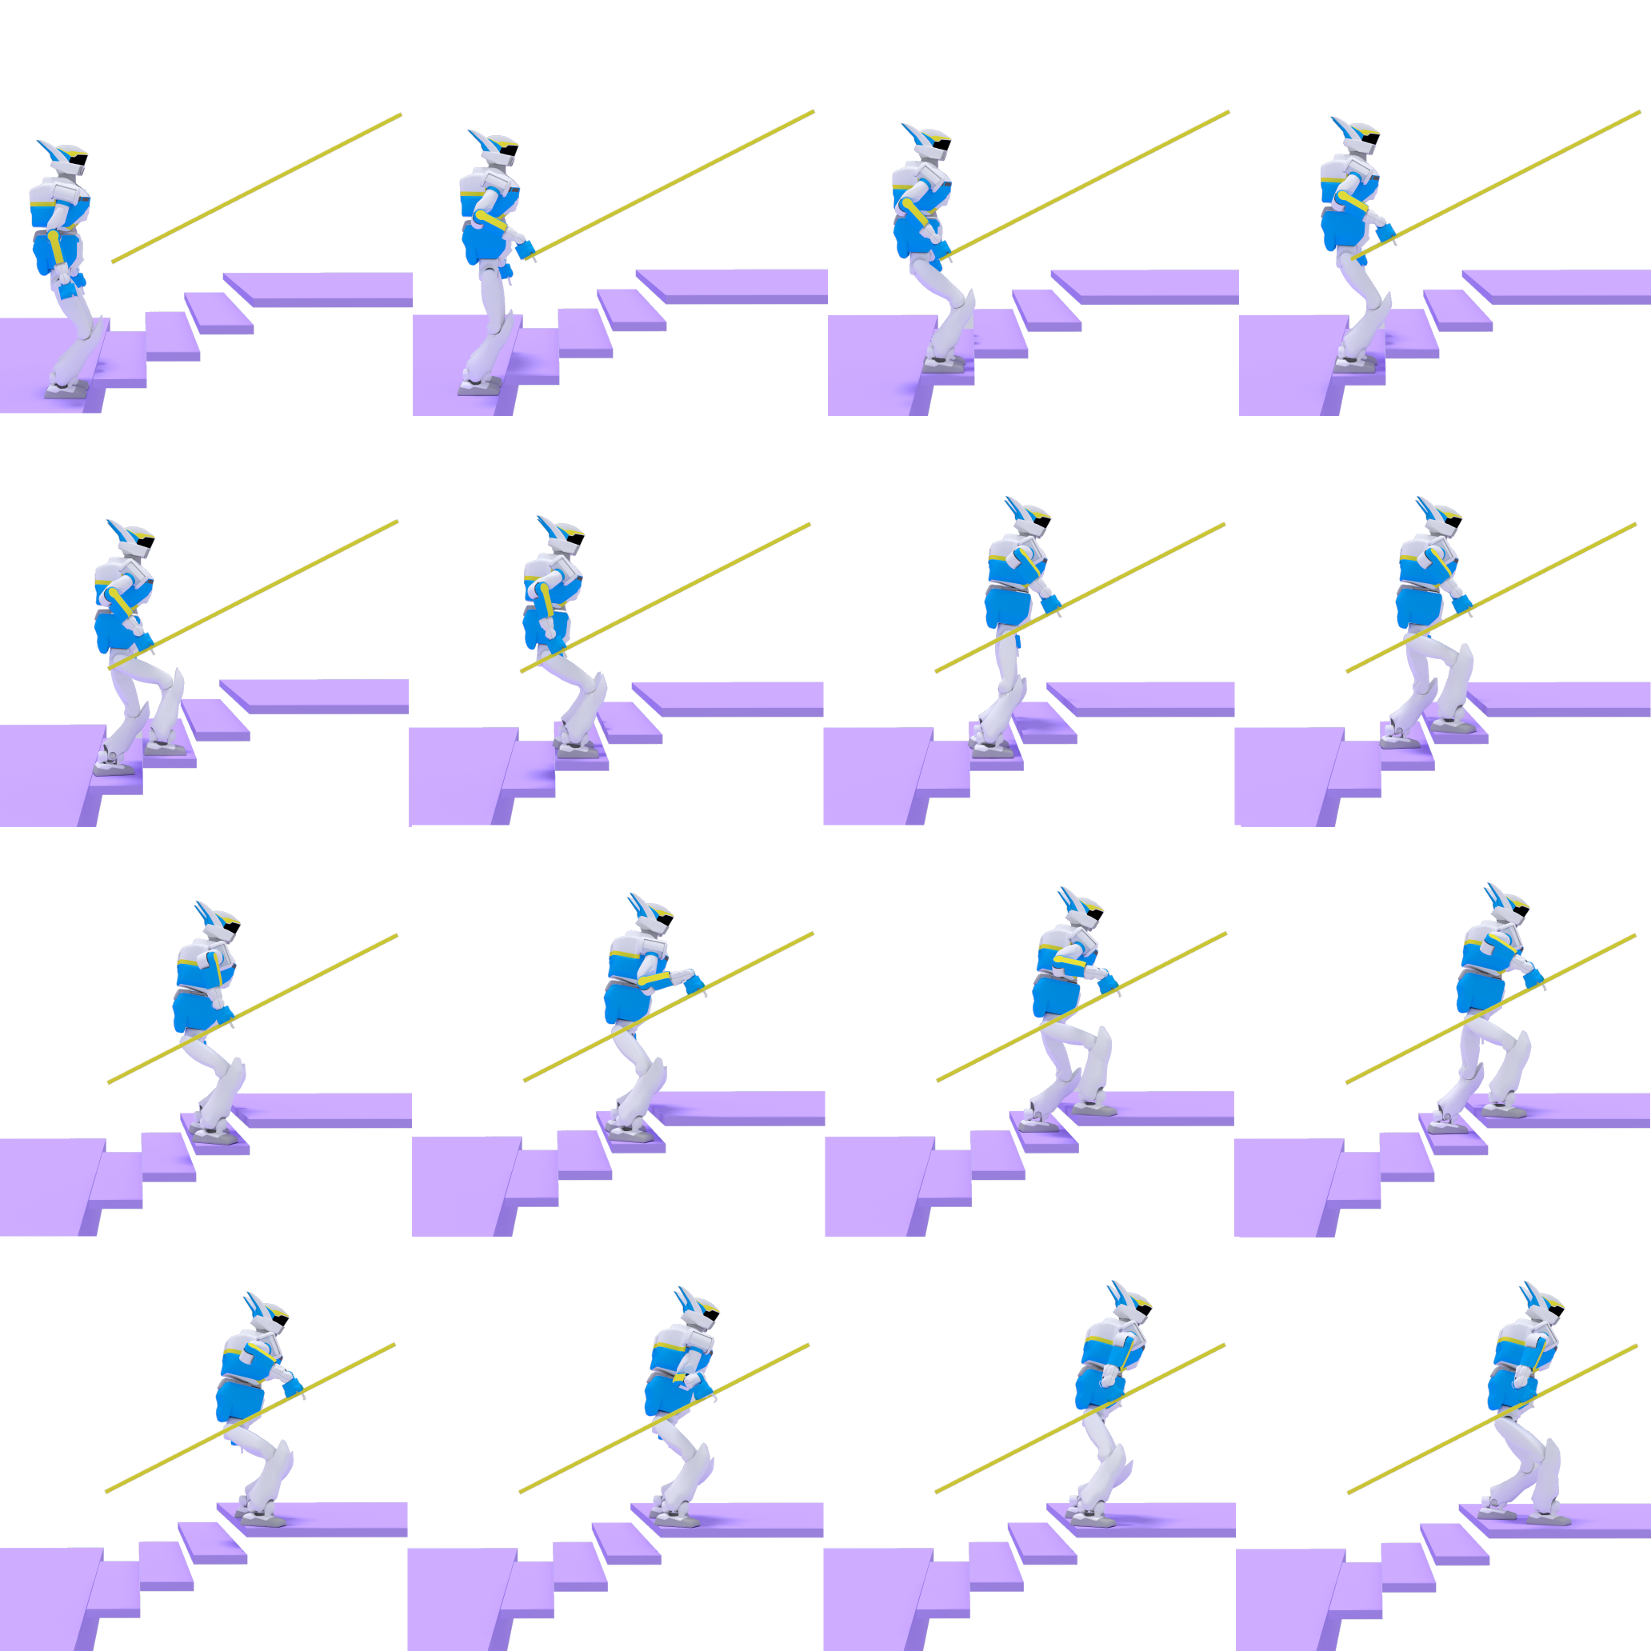
\includegraphics[width=1\linewidth]{figures/stair}
  \caption{
           HRP-2 in the steep stair climbing scenario. }
		   \label{fig:stair_robust}
\end{figure}

The goal is to climb three 15-cm high steps.

\noindent\textbf{Contacts involved:} Feet and right arm.

\noindent\textbf{Heuristics:} The manipulability $h_w$ is chosen for the feet; $h_{\textrm{\it EFORT}}$ is chosen for the right arm.
%~ Regarding equilibrium, the video demonstrates two sequences computed for two different threshold values of $b_0$: $0$ and $2$ (Figure~\ref{fig:stair_robust}). 

%~ \noindent\textbf{Observations:}
%~ This scenario illustrates best the importance of the equilibrium-robustness criterion.
%~ With a robust approach, more states are required to reach the last step (15 rather than 13 in average).
%~ However, when the last step is reached by both feet, in the nonrobust case the contacts are extremely close to 
%~ the cone limits (Figure~\ref{fig:stair_comp}).
%~ 
%~ 
%~ The geometry of the environment is easily addressed by our planner, and the contact planning is several times faster than real time in this scenario.
%~ 
%~ Again, the interpolation motion between the contact steps is out of the scope of this paper. However it should be noted that the computed plan in this scenario has been executed successfully on the robot (\url{http://youtu.be/YjL-DBQgXwk#t=0m28s}).
%~ 
%~ \begin{figure}
  %~ \centering
  %~ \begin{overpic}[width=0.5\linewidth]{figures/stair_robust}
		%~ \put (17,5) {\small{\color{red}$b_0 = 0.23$}} 
		%~ \put (79,5) {\small{\color{green}$b_0 = 6.16$}} 
	%~ \end{overpic}
  %~ \caption{
           %~ Evaluation of the robustness $b_0$ of two contact configurations. Although in equilibrium, the left configuration is on the verge of slipping.}
		   %~ \label{fig:stair_comp}
%~ \end{figure}

\subsubsection{HRP-2 -- Standing up (Figure~\ref{fig:standing}):}
From a bent configuration, the robot has to stand up using a wall as support, and climbing a 25-cm high step.

\begin{figure}
  \centering
  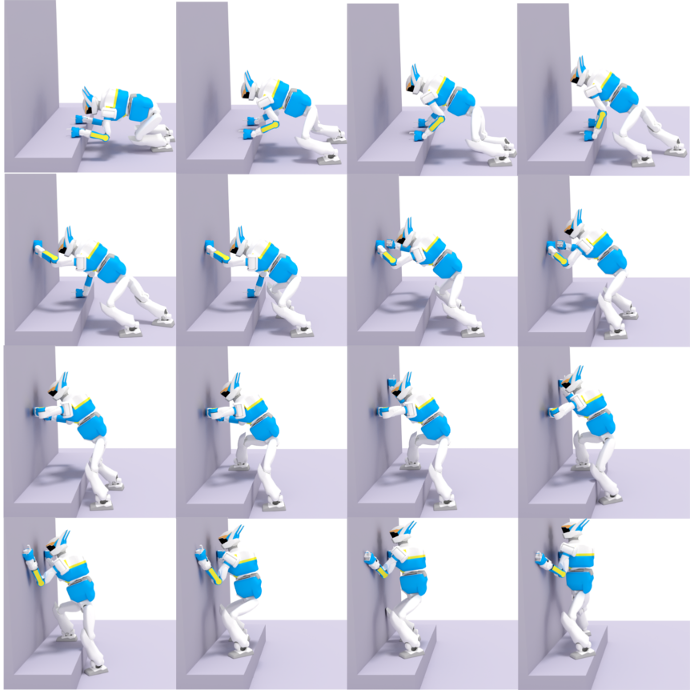
\includegraphics[width=1\linewidth]{figures/standing}
  \caption{
           HRP-2 in the standing scenario. }
		   \label{fig:standing}
\end{figure}


\noindent\textbf{Contacts involved:} All (both feet and hands).

\noindent\textbf{Heuristics:} $h_w$ for the feet, $h_{\textrm{\it EFORT}}$  for the hands.

%~ \noindent\textbf{Observations:} The scenario illustrates well the acyclic aspect of the planning. For instance, in the four first frames of Figure~\ref{fig:standing}, we can see that the right foot
%~ is moved twice, with the left foot in between, before the configuration allows HRP-2 to move its hand.
%~ Because the contacts are tried in a FIFO manner, the fact that the output contact sequence is acyclic shows that a cyclic approach (with a finite state machine for instance) is not sufficient
%~ for the computed path. The reason for this is not reachability, but equilibrium. The planning is slower than for the stair scenario (because the contact generation fails more),
%~ though it remains compatible with \gls{interactive} performances. % \adnote{Maybe define what you mean by 'interactive' and 'real-time' at some point.}


\subsubsection{HRP-2 -- Polaris car egress (Figure~\ref{fig:car}):}
In this scenario inspired from the DRC car egress HRP-2 has to step out of the Polaris car.

\begin{figure}
  \centering
  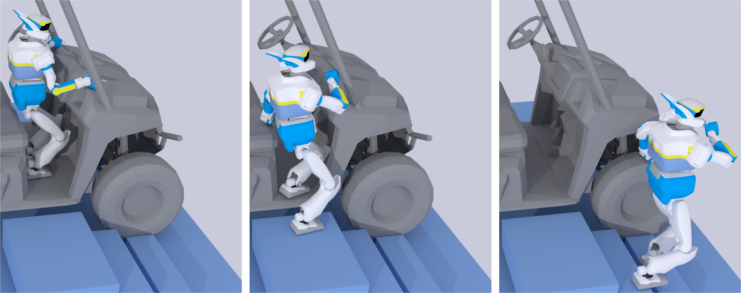
\includegraphics[width=1\linewidth]{figures/polaris}
  \caption{
           Selected frames from the polaris egress scenario. }
		   \label{fig:car}
\end{figure}


\noindent\textbf{Contacts involved:} All (both feet and hands).

\noindent\textbf{Heuristics:} $h_w$.

%~ \noindent\textbf{Observations:} The difficulty of this scenario lies in the strong reduction of the reachable workspace induced 
%~ by the extreme proximity of all obstacles. The planner is able to find a sequence, that consists in many steps.
%~ The proximity of the obstacles invalidate a large number of contact candidates because of collisions. To avoid breaking more than one contact between each step, the motion has to be decomposed into a large number of steps (61 in average).
%~ While this scenario is the slowest to solve, the planner still computes a solution \glslink{interactive}{interactively}.


\subsubsection{HyQ -- DRC-style rubble (Figure~\ref{fig:darpa})}
The quadruped robot must cross a rubble composed of bricks rotated at different angles and directions.

\begin{figure}
  \centering
  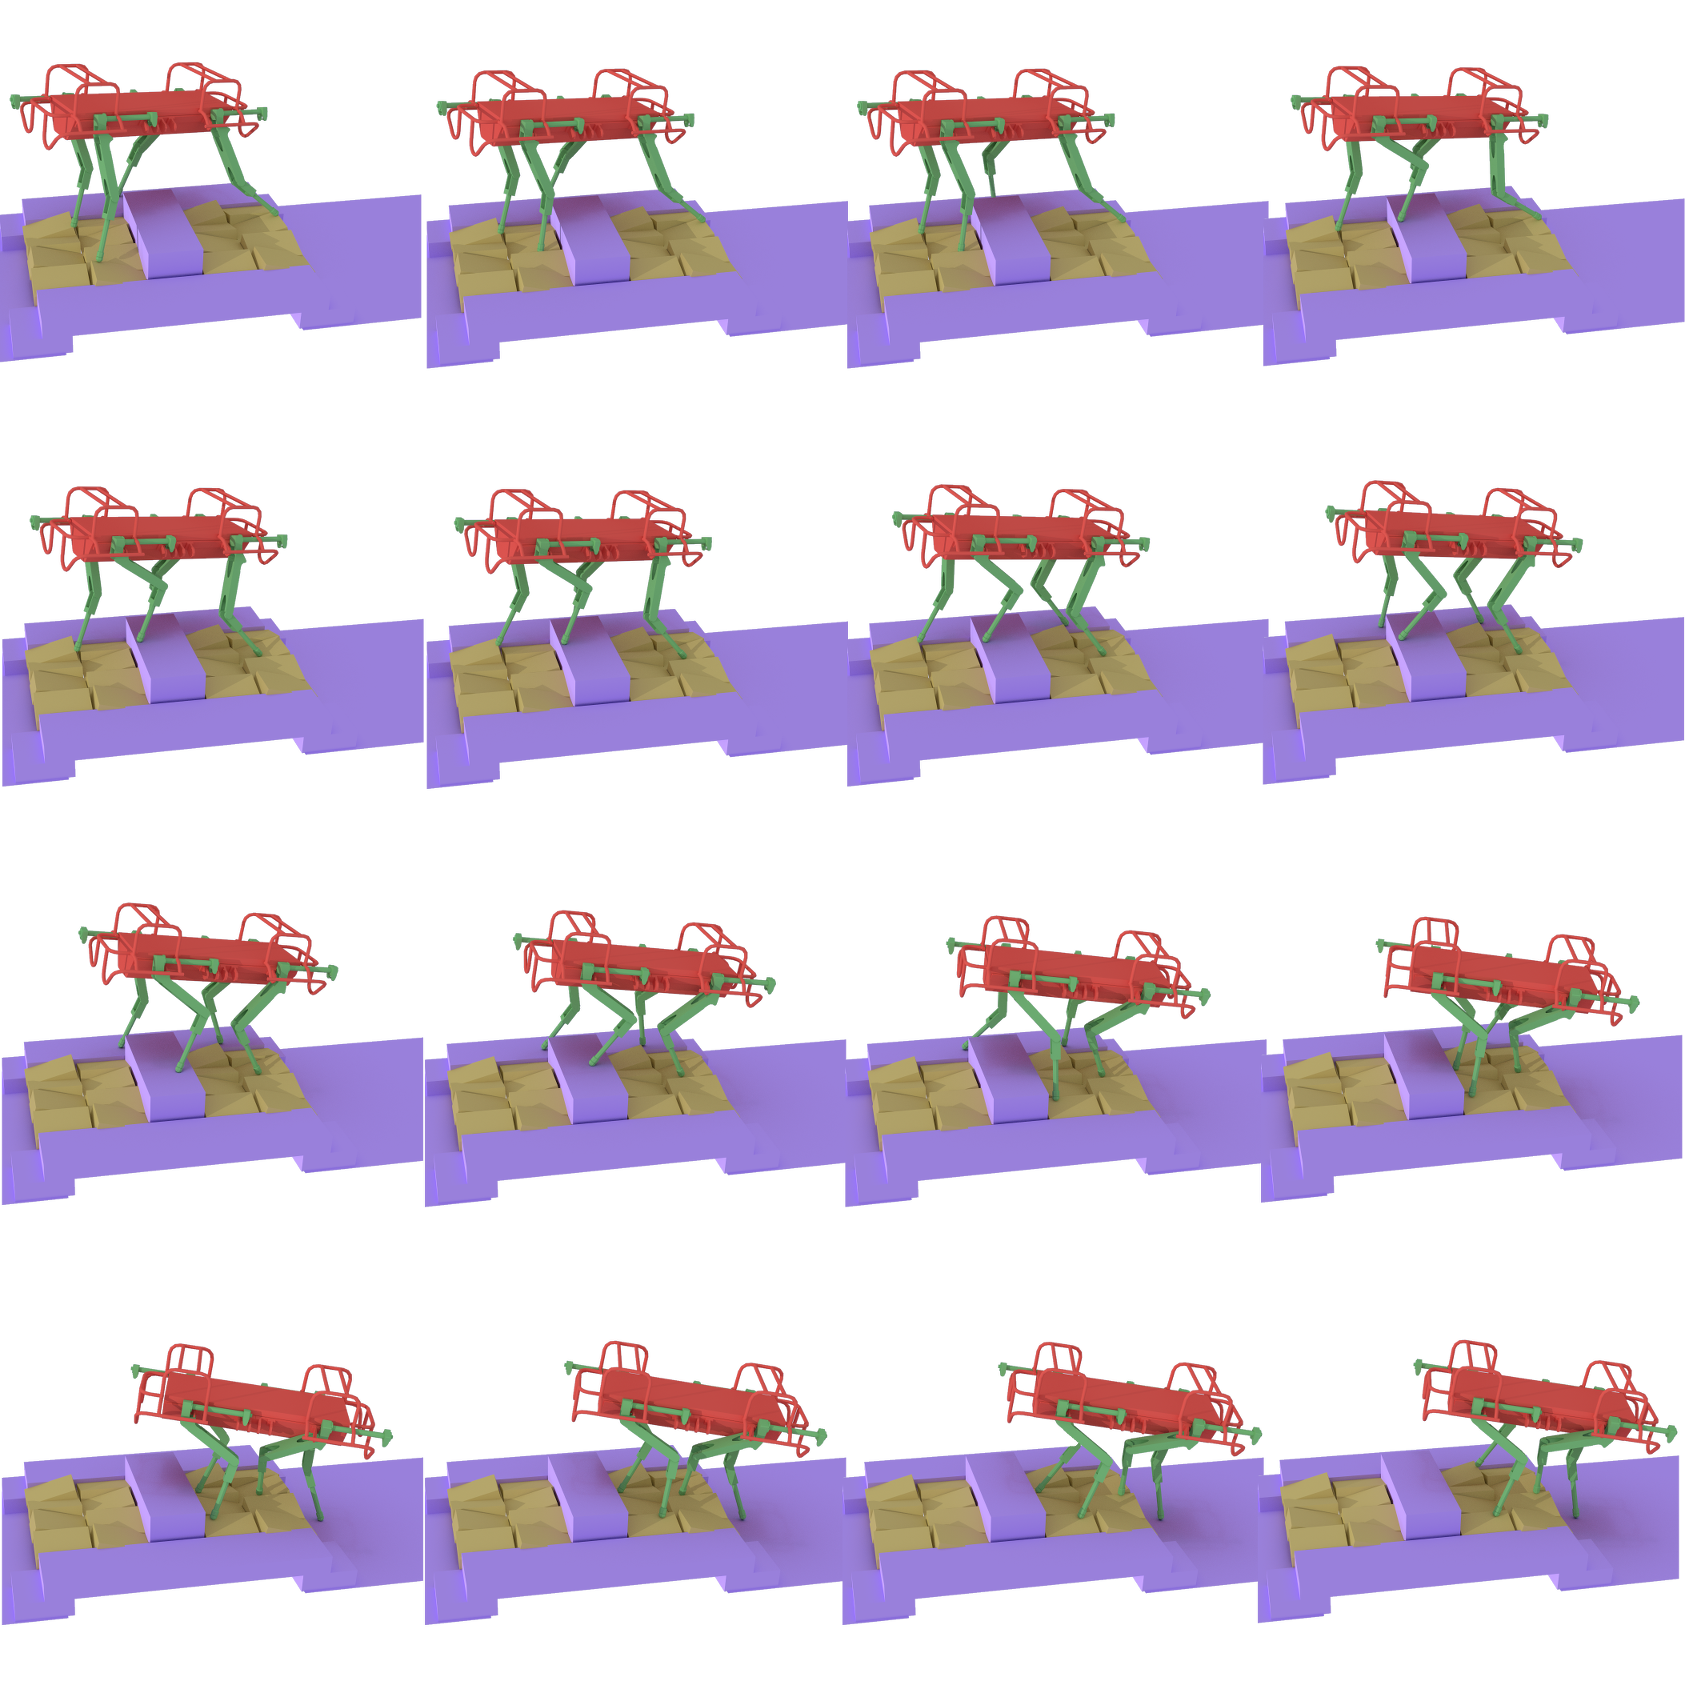
\includegraphics[width=1\linewidth]{figures/darpa}
  \caption{
           Robust crossing of rubbles by HyQ. }
		   \label{fig:darpa}
\end{figure}


\noindent\textbf{Contacts involved:} All (the 4 legs).

\noindent\textbf{Heuristics:} $h_w$ for all legs. The robustness threshold $b_0$ is set to $20$.

%~ \noindent\textbf{Observations:} In this context, setting up a really important minimum value for $b_0$ is possible due to the high
%~ stability of the HyQ robot, and results in more contact switches, in exchange for safety. The guide path-planning in this scenario takes a few seconds in average, more than
%~ in any other scenarios. This is explained by the necessity of discovering a safe way to ``climb down'' the rubble. In this part of the planning, the constraint that the 4 reachable workspaces of all legs must collide with the environment at all times is hard to respect, but enforces the equilibrium of HyQ. %\adnote{Why do not relax this constraint and require only 3 legs?} 
%~ Again, the computation times remain however \gls{interactive}.

\subsubsection{HyQ -- Obstacle race (Figure~\ref{fig:HyQ_bridge} and~\ref{fig:HyQ_obs}):}
In this long scene, HyQ has to cross a 55-cm large hole, followed by a narrow ``bridge'', only 25-cm large.

\begin{figure}
  \centering
  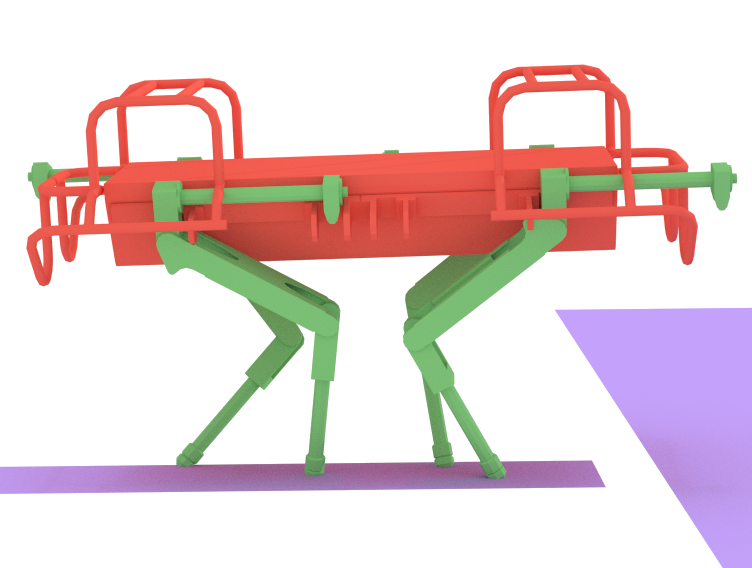
\includegraphics[width=0.4\linewidth]{figures/HyQ_bridge}
  \caption{
           HyQ crossing a narrow bridge. }
		   \label{fig:HyQ_bridge}
\end{figure}

\begin{figure}
  \centering
  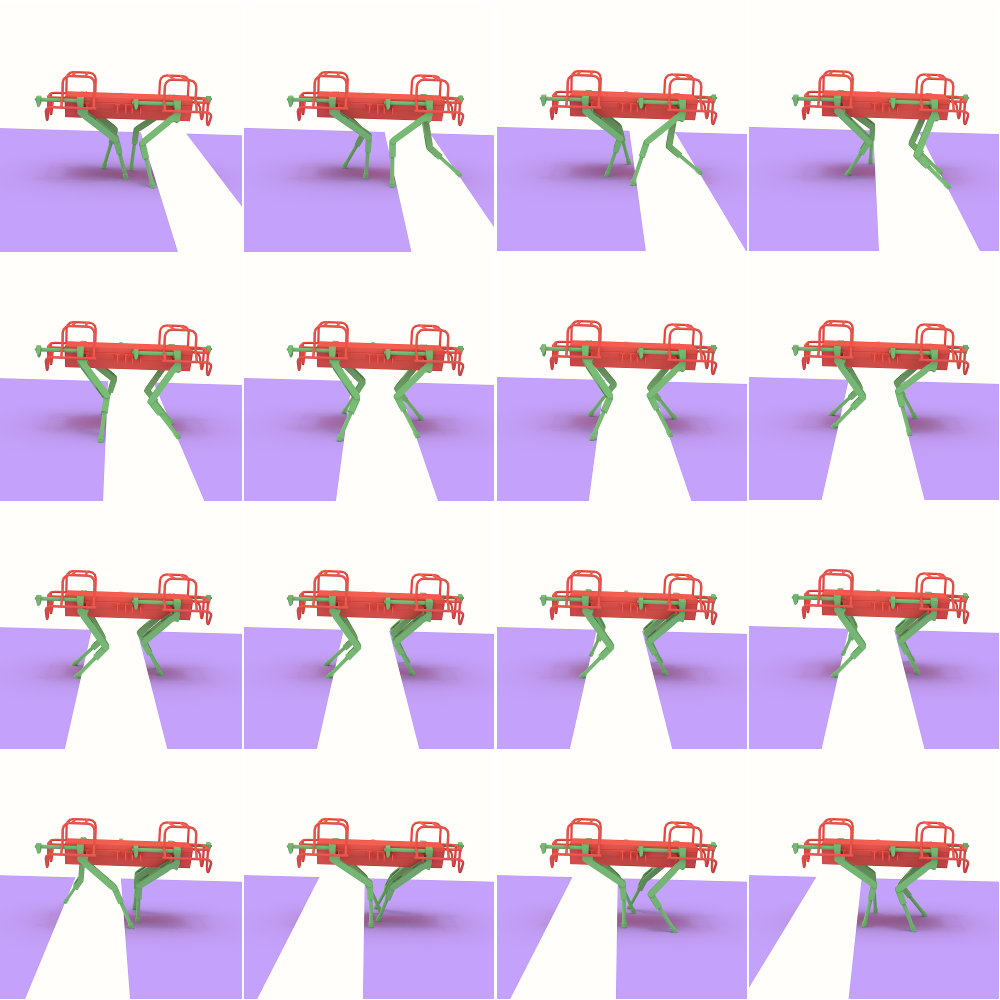
\includegraphics[width=1\linewidth]{figures/HyQ_obs}
  \caption{
           Crossing a hole contact sequence for HyQ. }
		   \label{fig:HyQ_obs}
\end{figure}



\noindent\textbf{Contacts involved:} All (the 4 legs).

\noindent\textbf{Heuristics:} $h_w$ for all legs. The robustness threshold $b_0$ is set to $10$.

%~ \noindent\textbf{Observations:} Despite the apparent simplicity of the scene, this scenario is a hard case for a contact planner.
%~ While finding a guide path above the hole is easy for the guide planner, finding a sequence of contacts that allows for equilibrium is not trivial.
%~ Second, the narrow bridge is hard both for the planner and the contact generator: to make sure that equilibrium is preserved along the traversal,
%~ the bridge must be approached with the appropriate angle.
%~ The difficulty is illustrated in Figure~\ref{fig:HyQ_obs}, where several feet rearrangements are required to cross the hole (although the video shows this best).
%~ The planner however succeeds in finding a feasible sequence in the end, again with \gls{interactive} computation times.

\subsubsection{HRP-2 -- Path re-planning (Figure~\ref{fig:re-planning}):}
In this long scene, HRP-2 plans a path through several obstacles. The scene is edited during the execution of the motion: a stair is added,
some stepping stones are removed, and part of the final staircase is deleted. All these modifications require re-planning.


\begin{figure}
  \centering
  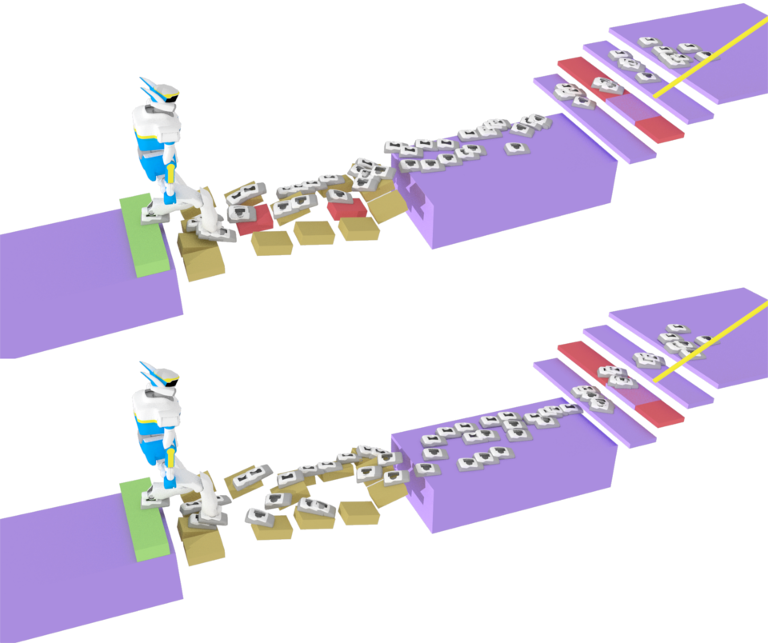
\includegraphics[width=0.7\linewidth]{figures/replanning}
  \caption{
           HRP-2 in the re-planning scenario. After the red step stones are removed, a new sequence of contacts is re-planned. Hand contacts
           are not presented here for readability.}
		   \label{fig:re-planning}
\end{figure}

\noindent\textbf{Contacts involved:} Feet and the right arm.

\noindent\textbf{Heuristics:} $h_w$  for all legs. $h_{\textrm{\it EFORT}}$  for the right arm. The robustness threshold is set to $2$.

%~ \noindent\textbf{Observations:} This scenario is designed to illustrate concretely the computation times of the planner.
%~ In the video, the footsteps indicating the contact sequence appear at the average speed of their computation (including the guide-path planning).


\subsubsection{3-fingered hand -- Manipulation of a pen (Figure~\ref{fig:penrot}):}
This scenario is proposed to illustrate the generality of our approach: we consider a manipulation task for a robotic hand and use
our contact planner to compute a contact sequence for the fingers, considered as effectors (Figure~\ref{fig:penrot}).
Although we do not address the hard issue of accounting for rolling motions, the planner is able to compute the shown sequences in less than 5 seconds.

\begin{figure*}
\centering
  \begin{overpic}[width=1\linewidth]{figures/penrot}
	\end{overpic}
\caption{Contact sequence found for a pen manipulation in a zero gravity environment.}
		   \label{fig:penrot}
\end{figure*}

 
\noindent\textbf{Contacts involved:} Three finger-tips.

\noindent\textbf{Heuristics:} $h_{\textrm{\it EFORT}}$ for all fingers.
 
 
\subsection{Role of the main parameters} \label{sec:influence}
We discuss the factors that influence the outcome of our planner: the root scaling factor $s$ (Section~\ref{sec:scaling}), the heuristics for
contact generation (Appendix~\ref{sec:heuristics}), and lastly, the discretization step for the guide path. The appropriate value for these parameters
is computed empirically based on use-case analysis or trials and errors.
 
\subsubsection{Choosing the scaling factor $s$} \label{sec:params}
%~ \deladp{To find a convenient value $s^*$ of $s$, we proceeded as follows. }
For several values of $s$, we generated $10 000$ configurations. 
We then computed the sensitivity of the reachability condition (percentage of configurations in $C_{Reach}^0$, effectively belonging to \gls{$C_{Contact}^0$}).
Similarly we computed the specificity of the condition (percentage of configurations \textbf{not} in $C_{Reach}^0$, effectively \textbf{not} belonging to \gls{$C_{Contact}^0$}).
The obtained results for HRP-2 are shown in Table~\ref{tab:scale}, averaged over all scenes (except for the car egress: in this scenario, 
statistical tests are not really conclusive since we are only interested in a small area of the environment).

As it can be expected, the scaling results in a high increase of the sensitivity, with a decrease of the specificity.
For HRP-2 we decided to set $s^*=1.2$.
%~ , and was also effective for the car egress scenario. 

\begin{table}
\centering
\footnotesize
\begin{tabular}{c | c | c}
   Value of $s$ &  Sensitivity & Specificity\\
 \hline
   1   & 76\% & 100 \%\\
   1.1& 88\% & 96\% \\
   1.15& 93\% & 94\%\\
   1.2 & 97\% & 92.5\%\\
   1.25& 98\% & 91.7\%\\
   1.5 & 99\% & 90.5\%\\
 \end{tabular}
\caption{Sensitivity and specificity values of the reachability condition, depending on the scaling value $s$ of $W^0$.}
\label{tab:scale}
\quad
\end{table}

\subsubsection{Choosing the heuristics} \label{sec:heuristichoices}
In our conference paper~\citep{tonneauisrr15}, the computed motions were generated using the EFORT heuristic.
EFORT is designed for tasks requiring to exert important forces (such as pushing / pulling / climbing). 
In locomotion tasks, such as the stair scenario, one issue with EFORT is that it tends to generate
configurations close to singularities (and joint limits). While this did not significantly impact
the generation of the plan, the resulting interpolation turned out to be harder.
For this reason, we prefer to use our manipulability-based heuristic for the legs of the robot, but we still
use EFORT for the arms, which results in fewer contact repositionings.

%~ \subsubsection{On the robustness equilibrium criterion:} \label{sec:parrob}
%~ Robustness is really important when considering practical applications on the robot, to account 
%~ for the various uncertainties that result from environment and state estimation. However,
%~ maximizing the robustness criterion is often not optimal, because the resulting configurations may be too conservative, thus not favoring the motion. In our experiments, we choose not to maximize the robustness,
%~ but to empirically se	t a robustness threshold value under which a configuration is not considered to be in
%~ static equilibrium (If no candidate reaches the threshold, instead of failing, the algorithm can eventually return the ``more robust'' configuration
%~ found). Currently for HRP-2, a threshold value of 2 subjectively gives the best results in the considered scenarios, while 10 seems to be a good choice for HyQ. Both values do not
%~ significantly slow down the planning times.

\subsubsection{Discretization of the guide path} \label{sec:disc}
The discretization step is a user-defined, fixed parameter. The step
has an influence on the output of the planner: if too large steps are taken,
the planner may fail since we impose the constraint that only one contact change might occur
between two consecutive steps. On the other hand, a small step will not impact the success rate of the planner, 
but may generate unnecessary states. In most scenarios the torso of HRP-2 moves about 15 cm between two postures, but only 3 cm
for the car egress scenario to handle the geometry of the polaris.
For future work, we would like to automatically adapt the size of the discretization step to the complexity of the environment.

\subsection{Performance analysis} \label{sec:perf}
To analyze performance, we ran the planner 1000 times for each considered scenario.
We measured the computation time spent in each part of the algorithm, and analyzed their success rate.


\begin{table*}
\centering
\footnotesize
\begin{tabular}{ >{\centering\arraybackslash}m{37pt} | >{\centering\arraybackslash}m{57pt} | >{\centering\arraybackslash}m{65pt} | >{\centering\arraybackslash}m{70pt} | >{\centering\arraybackslash}m{73pt} | >{\centering\arraybackslash}m{80pt} | >{\centering\arraybackslash}m{10pt}}
  Scenario (nb steps) &  Complete guide generation (ms) & Static equilibrium (ms) & Collision (ms) & Inverse Kinematics (ms) & Total generation time (ms) & Time per step (ms)\\
 \hline
   Stairs (18) 	& 5 -- \textbf{6} --  18 		 & 13 --  \textbf{32} -- 329   	& 1 --  \textbf{4} -- 38 & 26 --  \textbf{127} -- 1345 & 92 --  \textbf{261} -- 2174 & \textbf{15} \\
   Standing (24)& 65 -- \textbf{1086} --  5227   & 27 --  \textbf{144} -- 338   & 2 --  \textbf{12} -- 37 & 144 --  \textbf{1046} -- 2374 & 371 --  \textbf{2257} -- 7671 & \textbf{94}  \\
   Car (86)& 320 -- \textbf{6971} --  44002 & 409 --  \textbf{1766} -- 14752   	& 297 -- \textbf{1187} -- 8483 & 3154 --  \textbf{15323} -- 165541 & 5834 --  \textbf{31391} -- 281000 & \textbf{365}\\
   Rubble (82)& 37 -- \textbf{573} --  1685 & 583 --  \textbf{2714} -- 9459 & 491 --  \textbf{1971} -- 6273 & 269 --  \textbf{706} -- 3118 & 1811 --  \textbf{7195} -- 23241 & \textbf{86} \\
   Race (134)& 14 -- \textbf{51} --  125 & 455 --  \textbf{1359} -- 21045   & 397 --  \textbf{923} -- 9924 & 228 --  \textbf{471} -- 5415 & 1436 --  \textbf{3343} -- 41446 & \textbf{25}
 \end{tabular}
\caption{minimum, \textbf{average} and worst time (in ms) spent in the generation process for each scenario and each critical part of the generation process (not all parts are timed,
thus the average total computation time is higher than the sum of each part). The last
column indicates the average time necessary to compute one contact transition. }
\label{tab:requestime}
\quad
\end{table*}


\begin{table}
\centering
\begin{tabular}{ l | c}
  &  Path planning success rate \\
 \hline
   Stairs     	& 100\% \\
   Standing			& 68\% 	\\
   Car 			& 77\% 	\\
   Rubble 				& 97\% 	\\
   Race        & 88.0\% 	\\
 \end{tabular}
\caption{ Percentage of successful complete contact planning rates for each scenario, rounded to the first decimal.}
\label{tab:sucess_planning}
\quad
\end{table}

\begin{table}
\centering
\begin{tabular}{ l | >{\centering\arraybackslash}m{65pt} | >{\centering\arraybackslash}m{35pt} | >{\centering\arraybackslash}m{35pt} | c}
  &  Equilibrium success rate & Kinematic failure & Equilibrium failure \\
 \hline
   Steep stairs 	& 99.5\%  & 0.1\% 	& 0.4\% \\
   Standing up 		& 87.8\%  & 6.1\% 	& 6.1\% \\
   Car egress 		& 66.2\%  & 15.9\% 	& 17.9\% \\
   Rubble 			& 97.54\% & 0.16\% 	& 2.3\% \\
   Obstacle race 	& 92.4\%  & 0.15\% 	& 7.45\% \\
 \end{tabular}
\caption{Success rates obtained for the generation of static equilibrium contact configurations for each scenario, rounded to the first decimal. Column 1 indicates 
indicates the rate of contact generation that suceeeded. In the cases where the generation fails, it can be
either a kinematic issue (column 2), or because no contact configuration led to a static equilibrium configuration (column 3). Note that a failure in the contact generation
is not equivalent to a failure of the contact planning algorithm.}
\label{tab:requestpercent}
\quad
\end{table}

\subsubsection{Computation times:}
Table~\ref{tab:requestime} summarizes the computation times.

For HRP-2, most of the time was spent performing inverse kinematics.
This is not surprising considering the number of calls to the methods: IK projection is used intensively to maintain contact continuity between two postures; 
it is also applied every time a new candidate needs to be evaluated. In particular for the car egress scenario,
the kinematic constraints are very demanding to avoid collisions.

On the other hand for HyQ most of the time is spent testing the static equilibrium of the candidate configurations.

In all scenarios, one can observe that the average computation time for one single step is largely below one second,
thus allowing to consider \gls{interactive} applications and online autonomous planning of the robot motion.


\subsubsection{Success rates:}
Table~\ref{tab:sucess_planning} summarizes the successful planning rates.
Despite the complexity of the scenarios addressed, as well as the approximations made in our formulation, our planner succeeded in the large majority of cases.

Table~\ref{tab:requestpercent} presents the rate of successful contact generation. Note that a failure in contact generation for a root configuration is not equivalent to a failure in the contact plan. It simply means that another limb was tested for contact generation for the same root configuration.
As expected, the more constrained scenario, the car egress, provides the less satisfying results, despite the high success rate of the planner.

These results confirm that our approach provides a satisfying compromise between completeness and efficiency, thus allowing to consider online planning
while controlling the robot. Indeed, when the contact planning fails, it fails rapidly. This allows us to rapidly re-plan with a reasonable chance of success.
The most efficient (and immediate) approach to obtain a valid contact plan as fast as possible would be to launch in parallel several instances of the planner (our current implementation is single-threaded) and to use any successful result as a plan for solver $\mathcal{P}_3$.


\begin{table}
\centering
\begin{tabular}{ c | c | c }
 Scenario & Method  & Computation time \\
 \hline
   \multirow{3}{*}{Stair 20 cm} & Hauser~\cite{Hauser06usingmotion} &  5.42 min  \\							 
							  & Mordatch et al.\cite{Mordatch:2012:DCB:2185520.2185539} & 2 to 10 min \\
							 & \textbf{Ours} + \cite{Carpentier2016}  & \textbf{$ <$ 2s} \\
 \hline
   \multirow{3}{*}{Stair 30 cm} & Hauser~\cite{Hauser06usingmotion} &  4.08 min  \\
							 & Mordatch et al.\cite{Mordatch:2012:DCB:2185520.2185539} & 2 to 10 min \\
							 & \textbf{Ours}  & \textbf{$ <$ 2s}   \\
 \hline
   \multirow{3}{*}{Stair 40 cm} & Hauser \cite{Hauser06usingmotion} &  10.08 min  \\
							 & Mordatch et al.\cite{Mordatch:2012:DCB:2185520.2185539} & 2 to 10 min \\
							 & \textbf{Ours}   & \textbf{$ <$ 5s}   \\
 \hline
   \multirow{2}{*}{Table (car) egress} & Bouyarmane et al.~\cite{Bouyarmane2009, DBLP:conf/iser/EscandeKMG08} & 3.5 hours  \\
							 & \textbf{Ours}  & \textbf{$<$ 60 s} \\
							 
 \end{tabular}
\caption{Comparison between the computation times obtained by our method and previous ones for addressing the whole problem.}
\label{tab:compprev}
\quad
\end{table}

\subsection{Validation of the contact plans, and comparison with previous work} \label{sec:compa}
To validate our plans, we either use the framework proposed in \cite{Carpentier2016} or our own implementation of a $\mathcal{P}_3$ solver, detailed in Appendix~\ref{app:optim}.
The companion video shows the obtained motions.

Few contributions provided computation times on the complete problem. %, necessary to provide comparison between our approaches. 
Furthermore, $\mathcal{P}_3$ remains an open problem in the presence of obstacles. The only valid scenarios addressed completely in previous works are thus the stair-climbing scenarios of different heights proposed by Hauser in \cite{Hauser06usingmotion}, and the table-egress scenario by Escande et al. in~\cite{DBLP:conf/iser/EscandeKMG08}, which we consider to be of similar complexity with respect to the car-egress scenario (we did not consider the stairs in the scene). Both scenarios are tested with HRP-2.

Table~\ref{tab:compprev} presents the computation times for these scenarios, clearly demonstrating that our approach is order of magnitude faster than previous works.




 \section{Discussion and future work} 
\label{sec:conclusion}

In this paper we consider the \gls{cluttered} contact planning problem, formulated as two sub-problems that we address sequentially.
The first problem $\mathcal{P}_1$ consists in computing an \gls{equilibrium feasible} guide path for the root of the robot;
 the second problem $\mathcal{P}_2$ is the computation of a discrete sequence of whole-body configurations along the root path.

Our contribution to \Pa is the introduction of a low-dimensional space $C_{reach}$, an approximation of the space of \gls{equilibrium feasible} root configurations.
Thanks to the computationally efficient verification of the \gls{reachc}, we are able to solve \Pa much faster than previous approaches.

%~ Our contribution to \Pa is a generic characterization of the properties that the guide path must satisfy, in particular to enforce the completeness of the acyclic contact planner. 
Our contribution to \Pb is a fast contact generation scheme that can take into
account criteria to optimize user-defined properties.

Our results demonstrate that our method allows a pragmatic compromise between three 
criteria that are hard to conciliate: generality, performance, and quality of the solution, making it the first acyclic contact
planner compatible with \gls{interactive} applications.
%
\textbf{Regarding generality}, the \gls{reachc}, coupled with an approach based on limb decomposition, 
allows the method to address arbitrary multiped robots in \gls{cluttered} problems. The only pre-requisite is the specification 
of the volumes $W^0$.
%
\textbf{Regarding performance}, our framework is really efficient in addressing both \Pa and $\mathcal{P}_2$. This results in \gls{interactive} computation times.
%
\textbf{Regarding the quality of the paths}, the \gls{reachc} allows us to compute
\gls{equilibrium feasible} paths in all the presented scenarios, with low rejection rates.
As for \cite{Bouyarmane2009}, failures can still occur, due to the approximate condition used to compute the guide path.
The low computational burden of our framework however allows for fast re-planning in case of failure.
Furthermore because of this approximation, the guide search is not complete. The choice is deliberate, because we are convinced
that it is necessary to trade completeness for efficiency at all stages of the planner.
However, one direction for future work is to focus on a more accurate formulation of $C_{reach}^0$ to improve
the approximation.

Another limitation of the method is that it currently only applies to \gls{cluttered} problems.
However, it should first be noted that many problems belong to this class: for instance all the problems
at the DRC were \gls{cluttered}. Our method is thus already useful for many cases.
One way of extending its range of application, that we 
consider for future work, is to include the equilibrium criterion when solving $\mathcal{P}_1$.
Considering the set of obstacles intersecting with the reachable workspace for a given root configuration as candidates surfaces, we can use them to verify the equilibrium criterion.
This would give us a necessary condition for \equilibriumfeasibility.


Regarding the interpolation between the contact sequences ($\mathcal{P}_3$), we have already obtained some success for some of the computed sequences~\citep{Carpentier2016}, but additional
work is required on the planning side to obtain a seamless workflow. To achieve this, we are currently working on the notion of transition certificate, i.e. formulating
conditions that guarantee that the interpolation between two contact configurations is dynamically feasible.
%~ Our current direction is to propose a geometric quantification of both the kinematic and dynamic constraints of the problem, expressed
%~ at the center of mass of the robot.
 %~ We are also
%~ working on new heuristics more closely related to the dynamics of the systems (for instance, choose the contacts that minimize the jerk between two contact configurations).
A last limitation of our method is that only static equilibrium configurations are considered for contact planning.
We aim at performing kinodynamic planning to overcome this limitation. We believe that the most promising direction in this regard is to integrate
the notion of Admissible Velocity Propagation in our current work \citep{DBLP:conf/rss/PhamCN13}.
Addressing these two last issues is essential to bridge the gap between the planning and control aspects of multiped locomotion.



% An example of a floating figure using the graphicx package.
% Note that \label must occur AFTER (or within) \caption.
% For figures, \caption should occur after the \includegraphics.
% Note that IEEEtran v1.7 and later has special internal code that
% is designed to preserve the operation of \label within \caption
% even when the captionsoff option is in effect. However, because
% of issues like this, it may be the safest practice to put all your
% \label just after \caption rather than within \caption{}.
%
% Reminder: the "draftcls" or "draftclsnofoot", not "draft", class
% option should be used if it is desired that the figures are to be
% displayed while in draft mode.
%
%\begin{figure}[!t]
%\centering
%\includegraphics[width=2.5in]{myfigure}
% where an .eps filename suffix will be assumed under latex, 
% and a .pdf suffix will be assumed for pdflatex; or what has been declared
% via \DeclareGraphicsExtensions.
%\caption{Simulation results for the network.}
%\label{fig_sim}
%\end{figure}

% Note that the IEEE typically puts floats only at the top, even when this
% results in a large percentage of a column being occupied by floats.


% An example of a double column floating figure using two subfigures.
% (The subfig.sty package must be loaded for this to work.)
% The subfigure \label commands are set within each subfloat command,
% and the \label for the overall figure must come after \caption.
% \hfil is used as a separator to get equal spacing.
% Watch out that the combined width of all the subfigures on a 
% line do not exceed the text width or a line break will occur.
%
%\begin{figure*}[!t]
%\centering
%\subfloat[Case I]{\includegraphics[width=2.5in]{box}%
%\label{fig_first_case}}
%\hfil
%\subfloat[Case II]{\includegraphics[width=2.5in]{box}%
%\label{fig_second_case}}
%\caption{Simulation results for the network.}
%\label{fig_sim}
%\end{figure*}
%
% Note that often IEEE papers with subfigures do not employ subfigure
% captions (using the optional argument to \subfloat[]), but instead will
% reference/describe all of them (a), (b), etc., within the main caption.
% Be aware that for subfig.sty to generate the (a), (b), etc., subfigure
% labels, the optional argument to \subfloat must be present. If a
% subcaption is not desired, just leave its contents blank,
% e.g., \subfloat[].


% An example of a floating table. Note that, for IEEE style tables, the
% \caption command should come BEFORE the table and, given that table
% captions serve much like titles, are usually capitalized except for words
% such as a, an, and, as, at, but, by, for, in, nor, of, on, or, the, to
% and up, which are usually not capitalized unless they are the first or
% last word of the caption. Table text will default to \footnotesize as
% the IEEE normally uses this smaller font for tables.
% The \label must come after \caption as always.
%
%\begin{table}[!t]
%% increase table row spacing, adjust to taste
%\renewcommand{\arraystretch}{1.3}
% if using array.sty, it might be a good idea to tweak the value of
% \extrarowheight as needed to properly center the text within the cells
%\caption{An Example of a Table}
%\label{table_example}
%\centering
%% Some packages, such as MDW tools, offer better commands for making tables
%% than the plain LaTeX2e tabular which is used here.
%\begin{tabular}{|c||c|}
%\hline
%One & Two\\
%\hline
%Three & Four\\
%\hline
%\end{tabular}
%\end{table}


% Note that the IEEE does not put floats in the very first column
% - or typically anywhere on the first page for that matter. Also,
% in-text middle ("here") positioning is typically not used, but it
% is allowed and encouraged for Computer Society conferences (but
% not Computer Society journals). Most IEEE journals/conferences use
% top floats exclusively. 
% Note that, LaTeX2e, unlike IEEE journals/conferences, places
% footnotes above bottom floats. This can be corrected via the
% \fnbelowfloat command of the stfloats package.





% if have a single appendix:
%\appendix[Proof of the Zonklar Equations]
% or
%\appendix  % for no appendix heading
% do not use \section anymore after \appendix, only \section*
% is possibly needed

% use appendices with more than one appendix
% then use \section to start each appendix
% you must declare a \section before using any
% \subsection or using \label (\appendices by itself
% starts a section numbered zero.)
%


\appendices


% !TEX root =  ../main.tex

\subsection{A criterion for robust static equilibrium}
The planner is designed so that any generated contact configuration is in static equilibrium.
%~ Equilibrium is of course critical in legged locomotion. For this reason 
We are interested in a robust 
criterion, that ensures that the robot remains in equilibrium in a real-world application, regardless of perception and control uncertainties.

We first give a linear program (LP) that verifies whether a contact configuration allows for static equilibrium.
From this formulation we derive a new LP that quantifies the robustness of the equilibrium to uncertainties in the contact forces.
In turn, from this value we can either choose the most robust candidate, or set a threshold on the required robustness. While the presented LP is original, it is based on an analysis of the problem that we proposed in \citep{Prete2016}, where the interested reader can find more details.


\subsubsection{Conditions for static equilibrium}
We first define the variables of the problem, for $e$ contact points, expressed in world coordinates:
\begin{itemize}
\item $\mathbf{c} \in \mathbb{R}^3$ is the robot center of mass (COM);
%~ \item $\mathbf{L}  \in \mathbb{R}^3 $ is the angular momentum at the COM;
\item $m \in \mathbb{R}$ is the robot mass;
\item $\mathbf{g} = [0,0,-9.81]^T$ is the gravity acceleration;
\item $\mu$ is the friction coefficient;
\item for the i-th contact point $1 \leq i \leq e$:
	\begin{itemize}
	\item $\mathbf{p_i}$ is the contact position;
	\item $\mathbf{f_i}$ is the force applied at $\mathbf{p_i}$;
	\item $\mathbf{n}_i,\mathbf{\boldsymbol\upgamma}_{i1},\mathbf{\boldsymbol\upgamma}_{i2}$ form a local Cartesian coordinate system centered at $\mathbf{p_i}$. $\mathbf{n}_i$ is aligned
	with the contact surface normal, and the $\mathbf{\boldsymbol\upgamma}_i$s are tangent vectors.
	\end{itemize}
\end{itemize}

According to Coulomb's law, the nonslipping condition is verified if all the contact forces lie in the friction cone defined by the surface.
As classically done, we linearize the friction cone in a conservative fashion with a pyramid, described by four generating rays of unit length. We choose for instance:
\begin{equation*}
\mathbf{V}_{i} = \mat{\mathbf{n}_{i} + \mu \mathbf{\boldsymbol\upgamma}_{i1} & \mathbf{n}_{i} -\mu \mathbf{\boldsymbol\upgamma}_{i1} & \mathbf{n}_{i} + \mu \mathbf{\boldsymbol\upgamma}_{i2} & \mathbf{n}_{i} - \mu \mathbf{\boldsymbol\upgamma}_{i2}}^T
\end{equation*}

Any force belonging to the linearized cone
can thus be expressed as a positive combination of its four generating rays.
%~ \deleted{Therefore we can express the nonslipping constraint on $\mathbf{f}_i$ as:}

\begin{equation*}
\forall i  \qquad  \exists \bm{\beta}_i \in \mathbb{R}^{4} : \bm{\beta}_i \ge 0 \text{ and } \mathbf{f}_{i} = \mathbf{V}_{i} \bm{\beta}_i,
\end{equation*}
where $\bm{\beta}_i$ contains the coefficients of the cone generators.
We can then stack all the constraints to obtain:
\begin{equation}\label{eq:gen}
\exists \bm{\beta} \in \mathbb{R}^{4e} ,  \bm{\beta} \ge 0 \text{ and } \mathbf{f} = \mathbf{V} \bm{\beta},
\end{equation}
where $\mathbf{V} = \diag{ \{\mathbf{V}_1, \dots, \mathbf{V}_e\} }$, and $\mathbf{f} = (\mathbf{f}_0,...,\mathbf{f}_e)$.

From the Newton-Euler equations, to be in static equilibrium the contact forces have to compensate the gravitational forces:


%~ \begin{align}
%~ \underbrace{\mat{m (\ddot{\mathbf{c}} - \mathbf{g})  \\ m \mathbf{c} \times (\ddot{\mathbf{c}} - \mathbf{g}) + \dot{\mathbf{L}}}}_\mathbf{w}
%~ = 
%~ \underbrace{
%~ \mat{\mathbf{I}_3 & \dots & \mathbf{I}_3 \\
%~ \hat{\mathbf{p}}_1 & \dots & \hat{\mathbf{p}}_e} \mathbf{V}
%~ }_\mathbf{G}
%~ \bm{\beta},
%~ \end{align}
%~ where $\mathbf{w}\in \Rv{6}$ is the so-called gravito-inertial wrench (GIW) \citep{qiu:dhm:2011, Caron2015} and $\hat{\mathbf{p}} \in \R{3}{3}$ is the cross-product matrix associated to $\mathbf{p}$.

%~ Static balance assumes zero acceleration thus we can write:
\begin{align} \label{eq:new_eul}
\underbrace{
\mat{\mathbf{I}_3 & \dots & \mathbf{I}_3 \\
\hat{\mathbf{p}}_1 & \dots & \hat{\mathbf{p}}_e} \mathbf{V}
}_\mathbf{G} \bm{\beta}, = 
\underbrace{\mat{\mathbf{0}_{3\times 3} \\ m \hat{\mathbf{g}}}}_{\mathbf{D}} \mathbf{c} + 
\underbrace{\mat{-m\mathbf{g} \\ \mathbf{0}}}_{\mathbf{d}}
\end{align}
where $\hat{\mathbf{x}} \in \R{3}{3}$ is the cross-product matrix associated to $\mathbf{x}$.
%~ The right hand side of \eqref{eq:new_eul} is independent of $\mathbf{c}^z$ because of the cross product matrix $\hat{\mathbf{g}}$ inside $\mathbf{D}$, so we can rewrite it as: \adnote{It is not really necessary to show that equilibrium is independent of the com altitude here, anyway the com is given, not a variable, so it does not change the size of the problem}
%~ \begin{align} \label{eq:new_eul2d}
%~ \mathbf{w}_0 = \mathbf{D}^{xy} \mathbf{c}^{xy} + \mathbf{d}
%~ \end{align}

If there exists a $\bm{\beta}^*$ satisfying \eqref{eq:gen} and \eqref{eq:new_eul}, it means that the configuration is in static equilibrium.
The problem can then be formulated as an LP:

\begin{equation} \label{eq:lin_prog} \begin{aligned}
\find \quad & \bm{\beta} \in \Rv{4e} \\
%~ \st \quad &\mathbf{G} \bm{\beta} = \mathbf{D}^{xy} \mathbf{c}^{xy} + \mathbf{d} \\
\st \quad &\mathbf{G} \bm{\beta} = \mathbf{D} \mathbf{c} + \mathbf{d} \\
& \bm{\beta} \ge 0 \\
\end{aligned} \end{equation}

\subsubsection{Formulation of a robust LP}
Let $b_0 \in \mathbb{R}$ be a scalar value. We now define the following LP:

\begin{equation} \label{eq:lin_prog_rob} \begin{aligned}
\find \quad & \bm{\beta} \in \Rv{4e}, b_0 \in \Rv{} \\
\minimize  \quad & -b_0 \\
\st \quad &\mathbf{G} \bm{\beta} = \mathbf{D} \mathbf{c} + \mathbf{d} \\
%~ \st \quad &\mathbf{G} \bm{\beta} = \mathbf{D}^{xy} \mathbf{c}^{xy} + \mathbf{d} \\
& \bm{\beta} \ge b_0 \bm{1}\\
\end{aligned} \end{equation}

We observe that if $b_0$ is positive then \eqref{eq:lin_prog} admits a solution, and $b_0$ is proportional to the minimum distance of the contact forces to the boundaries of the friction cones.
If $b_0$ is negative, the configuration is not in static equilibrium, and $b_0$ indicates ``how far'' from equilibrium the configuration is. We thus use $b_0$ as a measure of robustness.

In our implementation, rather than solving directly \eqref{eq:lin_prog_rob}, we solve an equivalent problem of smaller dimension that we get by taking the dual of \eqref{eq:lin_prog_rob} and eliminating the Lagrange multipliers associated to the inequality constraints:
\begin{equation} \label{eq:dual} \begin{aligned}
\find \quad & \bm{\nu} \in \Rv{6}\\
\maximize  \quad & -(\mathbf{D} \mathbf{c} + \mathbf{d})^T \nu \\
\st \quad &\mathbf{G}^T \bm{\nu} \ge 0 \\
& \mathbf{1}^T \mathbf{G}^T \bm{\nu} = 1 \\
\end{aligned} \end{equation}

Indeed, from Slater's conditions \citep{Boyd:2004:CO:993483}, we know that the optimal values of an LP and its dual are equal. Thus the optimal value of the LP~\eqref{eq:dual} is indeed the optimal $b_0$.

%~ In conclusion, the LP~\eqref{eq:dual} provides a method to check rapidly static equilibrium, and returns a robustness value.
%~ This robustness criterion can be immediately transformed into a heuristic, and eventually be weighted with others.
%~ Another option to enforce robustness is to set a minimum acceptable value for $b_0$, but as a result this conservative approach discards valid solutions.

% !TEX root =  ../main.tex
\subsection{Manipulability-based heuristics for contact selection}
This Section proposes heuristics to select a contact that optimizes desired capabilities.
%~ These heuristics allow to locally optimize a contact location with respect to a particular task.
For instance, one can be interested in configurations that allow to efficiently exert a force in the global direction of motion,
a high velocity in a given direction, or to stay away from singular configurations.
We derive three such heuristics from the work by \cite{Yoshikawa1984}, recalled here. %, that we present first.

\subsubsection{The force and velocity ellipsoids:}

\begin{figure}[!tbp]
  \centering
	\begin{overpic}[width=1\linewidth]{figures/EFORT/ellipsoid}
		\put (8.5,1.2) {\small{Velocity ellipsoid}}
		\put (62.5,1.2) {\small{Force ellipsoid} \tiny{(scale 0.5)}}
	\end{overpic}
  \caption{Examples of velocity and force ellipsoids for a manipulator composed of 2 DoFs and 2 segments.
Only the horizontal and vertical speeds are shown (not the rotation speeds).}
 %~ since it would require being able to draw in four dimensions.}
		   \label{sec:efort_ellipsoid}
\end{figure}


We consider: a limb configuration $\mathbf{q}^k$; its end effector position $\mathbf{p}^k$; its Jacobian matrix
$\mathbf{J}^k(\mathbf{q}^k)$; a force $\mathbf{f}$ exerted by the end effector. For clarity in the rest of the section we omit the $k$ indices and write $\mathbf{J}^k(\mathbf{q}^k)$ as $\mathbf{J}$.
\citeauthor{Yoshikawa1984} defines the velocity~\ref{eq:vel} and force~\ref{eq:vel} ellipsoids:
 
 \begin{equation} 
 \label{eq:vel}
\mathbf{\dot{p}}^T(\mathbf{J}\mathbf{J}^T)^{-1}\mathbf{\dot{p}} \leq 1 
\end{equation}
 
 \begin{equation} 
 \label{eq:for}
\mathbf{f}^T (\mathbf{J}\mathbf{J}^T) \mathbf{f} \leq 1
\end{equation}

They describe the set of end-effector velocities (respectively forces) that can
be reached under the constraint $||\dot{\mathbf{q}}||^2 \leq 1$ for the current configuration.
The longer the axis of the ellipsoid is, the more important the velocity (resp. force) of the end-effector the direction of the axis can be (Figure~\ref{sec:efort_ellipsoid}).
 
%~ Similarly, \citeauthor{Yoshikawa1984} also defines the force ellipsoid (Figure~\ref{sec:efort_ellipsoid} - right):
 
%~ \begin{equation} \label{ellipsoidforce}
%~ \mathbf{f}^T (\mathbf{J}\mathbf{J}^T) \mathbf{f} \leq 1
%~ \end{equation}
%~ with $\mathbf{f}$ is a force vector expressed in the task space $\mathbb{R}^m$;

\subsubsection{Manipulability-based heuristics:}
From these definitions, we can derive three useful heuristics, that all account for the environment and the task being performed.
The first one, EFORT, was introduced by \cite{Tonneau2014}; the other two are new minor contributions, derived from these previous works.

With EFORT, we define the efficiency of a configuration as the ability of a limb to exert a force in a given direction.
We thus consider the force ellipsoid as a basis for our heuristic.
In a given direction $\mathbf{m}$, the length of the ellipsoid is given by the force-transmission ratio \citep{1087795}:
\begin{equation*}
f_\mathsf{T}(\mathbf{q}, \mathbf{m}) = [\mathbf{m}^{T}(\mathbf{J}\mathbf{J}	^{T})\mathbf{m}]^{-\frac{1}{2}}
\end{equation*}

In our problem, to compare candidate configurations, we include the quality of the contact surface, and choose $\mathbf{m}$ as the direction
opposite to the local motion (given by the difference between two consecutive root positions):

\begin{equation}
h_{\textrm{\it EFORT}}(\mathbf{q}, \mathbf{m}) = [\mathbf{m}^{T}(\mathbf{J}\mathbf{J}^T)\mathbf{m}]^{-\frac{1}{2}} ( \mu \mathbf{n}^T \mathbf{m})
\end{equation}
where $\mu$ and $\mathbf{n}$ are respectively the friction coefficient and the normal vector of the contact surface.


If the ability to generate large velocities at the effector is considered, we define a new heuristic $h_{vel}$ with a similar reasoning on the velocity ellipsoid:
\begin{equation}
h_{vel}(\mathbf{q}, \mathbf{m}) = [\mathbf{m}^{T}(\mathbf{J}\mathbf{J}^T)^{-1}\mathbf{m}]^{-\frac{1}{2}} ( \mu \mathbf{n}^T \mathbf{m})
\end{equation}

$h_{\textrm{\it EFORT}}$ and $h_{vel}$ will favor contacts that allow large efforts or fast modifications in the velocity.
$EFORT$ in particular is useful for tasks such as standing up, pushing / pulling.
In other less demanding cases, manipulability can also be considered to avoid singularities.
To do so, we can consider the manipulability measure $h_{w}$, also given by \citeauthor{Yoshikawa1984}:

\begin{equation} \label{ellipsoid}
h_{w}(\mathbf{q}) = \sqrt{det(\mathbf{J}\mathbf{J}^T)}
\end{equation}
$h_{w}$ measures the ``distance'' of a given configuration to singularity. When $h_{w}$ is equal to 0, the configuration is singular;
the greater $h_{w}$ is, the further away the configuration is from singularity.

%~ $h_{\textrm{\it EFORT}}$, $h_{vel}$ and $h_{w}$ define three kinematic heuristics, fast to compute (indeed, thanks to our sampling-based approach, the Jacobian and inverse products
%~ can be precomputed off-line), that allow the planner to select the best
%~ candidates according to user-defined criterion.




%~ This results in faster computation times, and a reduced number of overall contact switches.




%~ where the $\dot$ symbol represents the time derivative.  It describes the set of end-effector velocities that can
%~ be reached under the constraint \eqref{ball} for the current configuration.
%~ The longer the axis of the ellipsoid is, the faster the end-effector can move along the direction of the axis (Figure~\ref{sec:efort_ellipsoid}).
 %~ 
%~ Similarly, \citeauthor{Yoshikawa1984} also defines the force ellipsoid(Figure~\ref{sec:efort_ellipsoid} - right):
 %~ 
%~ \begin{equation} \label{ellipsoidforce}
%~ \mathbf{f}^T (\mathbf{J}\mathbf{J}^T) \mathbf{f} \leq 1
%~ \end{equation}
%~ where $\mathbf{f}$ is a force vector $\mathbf{f}$ expressed in the task space $\mathbb{R}^m$;
%~ the equivalent joint torque vector $\bm{\tau}$;
 %~ 
%~ \begin{equation} \label{jac}
%~ \mathbf{\dot{p}}^k = \mathbf{J}^k(\mathbf{q}^k) \dot{\mathbf{q}}^k
%~ \end{equation}
%~ 
%~ For clarity in the rest of the section we omit the $k$ indices and write $\mathbf{J}^k(\mathbf{q}^k)$ as $\mathbf{J}$.
 %~ 
%~ As a linear approximation of a forward-kinematics function, $\mathbf{J}$ describes how small
%~ variations from the configuration $\mathbf{q}$ affect the position vector $\mathbf{p}$.

%~ Now we consider the unit ball in the configuration space $C$ defined by the set of joint velocities
%~ for which the norm is at most 1:
%~ \begin{equation} \label{ball}
%~ ||\dot{\mathbf{q}}||^2 \leq 1
%~ \end{equation}
%~ 
%~ We assume that $\mathbf{J}$ is full rank (we are not interested in singular configurations, which we discard).
%~ From \eqref{jac} we can thus obtain the following equality (Appendix~\ref{app:manipulability}):
%~ \begin{equation} \label{jaceq}
%~ \mathbf{\dot{p}}^T(\mathbf{J}\mathbf{J}^T)^{-1}\mathbf{\dot{p}} = \dot{\mathbf{q}}^T \dot{\mathbf{q}}
%~ \end{equation}

%~ We can use \eqref{jaceq} to map the ball into an ellipsoid in the Euclidian space $\mathbb{R}^m$:

%~ \begin{equation} \label{ellipsoid}
%~ \mathbf{\dot{p}}^T(\mathbf{J}\mathbf{J}^T)^{-1}\mathbf{\dot{p}} \leq 1
%~ \end{equation}
%~ This ellipsoid is called the manipulability ellipsoid, or velocity ellipsoid, introduced by \cite{Yoshikawa1984}. It describes the set of end-effector velocities that can
%~ be reached under the constraint \eqref{ball} for the current configuration.
%~ The longer the axis of the ellipsoid is, the faster the end-effector can move along the direction of the axis.
%~ Figure~\ref{sec:efort_ellipsoid} - left shows the velocity ellipsoid for different configurations of a manipulator with two degrees of freedom.

%~ \begin{figure}[!tbp]
  %~ \centering
	%~ \begin{overpic}[width=1\linewidth]{figures/EFORT/ellipsoid}
		%~ \put (8.5,1.2) {\small{Velocity ellipsoid}}
		%~ \put (62.5,1.2) {\small{Force ellipsoid} \tiny{(scale 0.5)}}
	%~ \end{overpic}
  %~ \caption{Examples of velocity and force ellipsoids for a manipulator composed of 2 dofs and 2 segments.
%~ Only the horizontal and vertical speeds are shown (not the rotation speeds), since it would require being able to draw in four dimensions.}
		   %~ \label{sec:efort_ellipsoid}
%~ \end{figure}


%~ Similarly to the velocity ellipsoid, \citeauthor{Yoshikawa1984} also defines the force ellipsoid.
%~ Considering: a force vector $\mathbf{f}$ expressed in the task space $\mathbb{R}^m$;
%~ the equivalent joint torque vector $\bm{\tau}$;
%~ we can define the mechanical work in both spaces:
%~ \begin{equation*} \label{power}
%~ \dot{\mathbf{q}}^T \bm{\tau} = \dot{\mathbf{p}}^T \mathbf{f}
%~ \end{equation*}
%~ 
%~ 
%~ Exploiting \eqref{jac}, we can easily see that the set of achievable forces in $\mathbb{R}^m$ subject to the constraint:
%~ \begin{equation*} \label{ballforce}
%~ ||\bm{\tau}||^2 \leq 1
%~ \end{equation*}
%~ is the so-called force ellipsoid (Figure~\ref{sec:efort_ellipsoid} - right):
%~ \begin{equation} \label{ellipsoidforce}
%~ \mathbf{f}^T (\mathbf{J}\mathbf{J}^T) \mathbf{f} \leq 1
%~ \end{equation}

%~ \clearpage
\section{Generating the $W$ volumes for HRP-2}
\label{app:rom}

We detail our method to generate the volumes $W$ used
in RB-RRT, with the example of HRP-2.
The kinematic tree is split into four limbs $R^k$.
The arms are connected to the shoulders, and the legs to the root.
The obtained volumes $W$ are shown in Figure~\ref{fig:hrp2_w}.

\begin{figure}
\centering
  \begin{overpic}[width=1\linewidth]{figures/hrp2_w}
	\end{overpic}
\caption{The $W$ volumes computed for HRP-2. The red shapes are $W^0$. The green shapes represent the $W^k$.}
		   \label{fig:hrp2_w}
\end{figure}

\subsection{Step 1: computing the reachable workspace $W^k$ of a limb}


To generate a volume $W^k$, we proceed as follows:
\begin{enumerate}
\item Generate randomly $N$ valid limb configurations for $R^k$, for $N$ really large (say $100000$);
\item For each configuration, store the 3D position of the end effector joint relatively to the root of $R^k$; then compute the convex hull of the resulting point cloud;
\item The resulting polytope can contain a very large number of faces. A last step is thus to simplify it with the blender decimate tool (\url{http://wiki.blender.org/index.php/Doc:2.4/Manual/Modifiers/Generate/Decimate}). This tool removes a user-defined amount of vertices (and faces) of the polytope, thus resulting
in a conservative approximation of the original shape. For HRP-2 we apply the operator with a ratio of $0.06$, resulting in a polytope of 38 faces for the arms and the legs.
\end{enumerate}
  
\begin{figure}
\centering
  \begin{overpic}[width=1\linewidth]{figures/roms}
	\end{overpic}
\caption{Different approximations of the range of motion of the right arm of HRP-2. Left: non convex-hull, computed with the powercrust algorithm~\citep{Amenta:2001:PC:376957.376986}. Middle:
convex hull of the reachable workspace. Right: Simplified hull used in our experiments.}
		   \label{fig:hrp2_roms}
\end{figure}

Figure~\ref{fig:hrp2_roms} illustrate the obtained $W^k$ for HRP-2.
Regarding the procedure, we can see that step 2 is conservative (Figure~\ref{fig:hrp2_roms}--right), which 
is acceptable, especially because the lost set essentially relates to configurations close to singularity (they are close to the boundaries of the reachable workspace, and
often not \gls{contact reachable}, as illustrated in Figure~\ref{fig:dedefeas}, where the exterior boundaries of the reachable workspace appear
red, thus not belonging to $C_{Contact}^0$). We choose again to be less complete but more efficient, regarding the number of collision tests to be performed by RB-RRT.
In step 1 on the other hand, selecting the convex hull (Figure~\ref{fig:hrp2_roms}--middle) instead of a minimum encompassing shape (Figure~\ref{fig:hrp2_roms}--left) may introduce false positives.
Concretely, because the false positive set intersects with $W^0$, the scaling volume of the robot torso, the induced error is compensated,
as verified by the results shown by Table~\ref{tab:requestpercent}.

\subsection{Step 2: computing the torso scaling workspace $W^0$ of the robot}
To define the volume $W^0$ of HRP-2, we proceed in an empirical manner.
First, we compute the bounding boxes of the robot torso, head, and upper legs (Figure~\ref{fig:hrp2_w} -- red shapes).
Then, we perform a scaling of these boxes by a factor $s$. 
The higher $s$ is, the more likely sampled configurations are to be feasible, but the less complete is the approach.
To compute the appropriate value of $s$, we proceed as described in Section~\ref{sec:params}, and choose empirically
$s^*=1.2$ as the appropriate value for HRP-2.

\section{Algorithms for discretizing of a path}
\label{app:contact}


First, we define an abtract structure State,
that describes a contact configuration.
The use of queues allows a FIFO approach regarding the order 
in which contacts are tested: we try to replace older contacts first when necessary.
Thus the algorithm is deterministic even though it can handle acyclic motions.

\begin{lstlisting}]
Struct Limb
{
    // Limb Configuration
    Configuration qk;
    // Effector position in
    // world coordinates
    vector6 pk;
};

Struct State
{
    // root location
    Configuration q0;
    // List of limbs not in contact
    queue<Limb> freeLimbs;
    // List of limbs in contact
    queue<Limb> contactLimbs;
};
\end{lstlisting}

From the start configuration, given as an input by the user,
we create the initial state $s0$.
Algorithm~\ref{alg:interpolate}  is then called with $s0$, as well as the discretized path 
$\mathbf{Q}^0$, as input parameters.

\begin{algorithm}
\caption{Discretization of a path} \label{interpolate}
	\begin{algorithmic}[1]
	%~ \Function{GenerateConfiguration}{}
	\Function{Interpolate}{$s0$,$\mathbf{Q}^0$, $MAX\_TRIES$}
		\State $list<$State$>$ $states = [s0]$
		\State $nb\_fail = 0$ 
		\State $i = 1;$ /*Current index in the list*/
		\While {$i < length(\mathbf{Q}^0)$}
			\State State $previous = last\_element(states)$
			\State State $s = \pi(previous, \mathbf{Q}^0[i])$
			\If {$s != NULL $}
				\State $nb\_fail = 0$
				\State $i += 1$
				\State \textbf{return} $\mathbf{q}^{0}$
			\Else
				\State $nb\_fail += 1$
				\If {$nb\_fail == MAX\_TRIES$}
					\State \textbf{return} $FAILURE$
				\EndIf				
				\State $s = $\textsc{RepositionContacts}$(previous)$
			\EndIf
			\State $push\_back(states, s)$
		\EndWhile
		\State \textbf{return} $states$
	\EndFunction
\end{algorithmic}
\label{alg:interpolate}
\end{algorithm}

At each step, $g$ is called with the previous state as a parameter, as well
as a new root placement. $g$ returns a new contact configuration, if it suceeded
in computing a configuration with only one contact switch occuring.
If $g$ failed in achieving this, the method \textsc{RepositionContacts} is called.
It repositions one end effector (either a free limb, or the oldest active contact) towards a new contact position if possible.
This repositionning allows to increase the odds that the contact can be maintained at the next step.

The pseudo code for the method $g$ is given by Algorithm~\ref{alg:pi}.

\begin{algorithm}
\caption{Full body contact generation method} \label{interpolate}
	\begin{algorithmic}[1]
	%~ \Function{GenerateConfiguration}{}
	\Function{$g$}{$pState$,$\mathbf{q}^0$}
		\State State $newState$
		\State $newState.q0 = \mathbf{q}^0$
		\State $newState.freeLimbs = pState.freeLimbs$
		\State /*First try to maintain previous contacts*/
		\State $nbContactsBroken = 0$
		\For {\textbf{each} Limb $k$ in $previous.contactLimbs$}
			\If {$!$\textsc{MaintainContact}$(pState,\mathbf{q}^0,k)$}
				\State $nbContactsBroken += 1$
				\If {$nbContactsBroken > 1$}				
					\State \textbf{return} $NULL$
				\EndIf				
				\State $push(newState.freeLimbs,k)$
			\Else 					
				\State $push(newState.contactLimbs,k)$
			\EndIf
		\EndFor
		\For {\textbf{each} Limb $k$ in $previous.freeLimbs$}
			\If {\textsc{GenerateContact}$(\mathbf{q}^0,k)$}	
				\State $push(newState.contactLimbs,k)$			
				\State \textbf{return} $newState$
			\EndIf
		\EndFor
		\State \textbf{return} $NULL$
	\EndFunction
\end{algorithmic}
\label{alg:pi}
\end{algorithm}

The method \textsc{MaintainContact}$(pState,\mathbf{q}^0,k)$ performs inverse kinematics to reach the previous contact position for the Limb.
If it succeeds, the new limb configuration is assigned to $k$. If it fails, a random collision free configuration is assigned to $k$.

\textsc{GenerateContact}$(\mathbf{q}^0,k)$ is a call to the contact generator presented in Section~\ref{sec:single_contact}. It generates a contact configuration in static equilibrium, and assigns the corresponding configuration to $k$.
If it fails, $k$ remains unchanged if it is collision free, otherwise it is assigned a random collision free configuration.


The pseudo code for the method \textsc{RepositionContacts} is given by Algorithm~\ref{alg:repo}.


\begin{algorithm}
\caption{Performs contact repositioning for one limb} \label{interpolate}
	\begin{algorithmic}[1]
	\Function{RepositionContacts}{$state$}
		\State $i=0$
		\While {$i<length(states.freeLimbs)$}
			\State Limb $k = pop(states.freeLimbs)$
			\If {\textsc{GenerateContact}$(state.q0,k)$}	
				\State $push(newState.contactLimbs,k)$			
				\State \textbf{return}
			\Else
				\State $i+=1$
				\State $push(states.freeLimbs,k)$		
			\EndIf
		\EndWhile
		\State $i=0$
		\While {$i<length(states.contactLimbs)$}
			\State Limb $k = pop(states.contactLimbs)$
			\State Limb $copy = k$
			\State $i+=1$
			\If {\textsc{GenerateContact}$(state.q0,k)$}	
				\State $push(newState.contactLimbs,k)$			
				\State \textbf{return}
			\Else
				\State $push(newState.contactLimbs,copy)$	
			\EndIf
		\EndWhile
		/*Fails if impossible to relocate any effector*/
		\State \textbf{return} $FAILURE$
	\EndFunction
\end{algorithmic}
\label{alg:repo}
\end{algorithm}



\section{Source code of our planner}
\label{app:hpp}
Our planner is implemented using the Humanoid Path Planner (HPP) software.
HPP is an open source motion planning framework developed by the Gepetto team at LAAS-CNRS, that can be found at \url{http://projects.laas.fr/gepetto/index.php/Software/Main}.
The HPP modules implement the standard tools and algorithms used in motion planning,
such as the Bi-RRT planner from which RB-RRT is derived.

The robot models used in our experiments are described using the standard urdf file format, that is 
compatible with HPP.

Our implementation of the planner is also open source, and can be found at \url{https://github.com/stonneau/hpp-rbprm}. 
Contrary to the mature HPP, at the time of submitting this article,
our planner is not officialy released, mostly for lack of a complete documentation and a tutorial.

However a reader familiar with HPP should be able to use the library.
Our goal is to make our code useful for the community, and we are working on releasing a stable 
version of our planner as soon as possible.



\section*{Acknowledgements}
This research is supported by Euroc (project under FP7 Grant Agreement  608849);  Entracte (ANR  grant  agreement  13-CORD-002-01);
the ARO Contract W911NF-14-1-0437; and the NSF award 1305286. %, and a grant from Boeing.


% can use a bibliography generated by BibTeX as a .bbl file
% BibTeX documentation can be easily obtained at:
% http://mirror.ctan.org/biblio/bibtex/contrib/doc/
% The IEEEtran BibTeX style support page is at:
% http://www.michaelshell.org/tex/ieeetran/bibtex/
\bibliographystyle{IEEEtran}
 %~ argument is your BibTeX string definitions and bibliography database(s)
\bibliography{biblio}
%
% <OR> manually copy in the resultant .bbl file
% set second argument of \begin to the number of references
% (used to reserve space for the reference number labels box)
%~ \begin{thebibliography}{1}
%~ 
%~ \bibitem{IEEEhowto:kopka}
%~ H.~Kopka and P.~W. Daly, \emph{A Guide to \LaTeX}, 3rd~ed.\hskip 1em plus
  %~ 0.5em minus 0.4em\relax Harlow, England: Addison-Wesley, 1999.
%~ 
%~ \end{thebibliography}



% biography section
% 
% If you have an EPS/PDF photo (graphicx package needed) extra braces are
% needed around the contents of the optional argument to biography to prevent
% the LaTeX parser from getting confused when it sees the complicated
% \includegraphics command within an optional argument. (You could create
% your own custom macro containing the \includegraphics command to make things
% simpler here.)
%\begin{IEEEbiography}[{\includegraphics[width=1in,height=1.25in,clip,keepaspectratio]{mshell}}]{Michael Shell}
% or if you just want to reserve a space for a photo:

\begin{IEEEbiographynophoto}{Steve Tonneau}
TODO
\end{IEEEbiographynophoto}

% insert where needed to balance the two columns on the last page with
% biographies
%\newpage

%~ \begin{IEEEbiographynophoto}{Jane Doe}
%~ Biography text here.
%~ \end{IEEEbiographynophoto}

% You can push biographies down or up by placing
% a \vfill before or after them. The appropriate
% use of \vfill depends on what kind of text is
% on the last page and whether or not the columns
% are being equalized.

%\vfill

% Can be used to pull up biographies so that the bottom of the last one
% is flush with the other column.
%\enlargethispage{-5in}



% that's all folks
\end{document}


